\documentclass[11pt,a4paper]{article}
\usepackage[utf8]{inputenc}
\usepackage[german]{babel}
\usepackage[T1]{fontenc}
\usepackage{amsmath}
\usepackage{amsfonts}
\usepackage{amssymb}
\usepackage{graphicx}
\usepackage[margin=1.25cm]{geometry} % Puts the same margin on all borders of the document

% Packages

\usepackage{hyperref} % Generate hyperlinks to referenced items
\usepackage{adjustbox} % Used to change parameters in \includegraphics[scale=•]{•}
\usepackage{enumitem} % Provides several options for lists
\usepackage{verbatim} % Package to use \begin{comment}
\usepackage{pdfpages} % Used to import PDF pages
\usepackage{multirow} % Allows us to have a single cell in a table span multiple rows
\usepackage{makecell} % Allows us to format multiple lines in a single cell
\usepackage{minted} % Used to syntax highlight code
\usepackage{xcolor}  % Gives access to coloring text
\usepackage{longtable} % Allows us to create a table over multiple pages
\usepackage{float} % Improved placement of floating items
\usepackage{pdfpages} % Used to import pdf pages
\usepackage{booktabs} % Used for horizontal lines instead of \hline



% Settings

\graphicspath{{./files/}} % Sets path for files to the files folder in the same directory

\hypersetup{
    colorlinks=false, %set true if you want colored links
    linktoc=all,     %set to all if you want both sections and subsections linked
    linkcolor=blue,  %choose some color if you want links to stand out
}


\renewcommand{\arraystretch}{1.75} 

\lstset {
	literate={~} {$\sim$}{1},
    language=Java,
    basicstyle=\footnotesize,
    numbers=left,
    stepnumber=1,
    showstringspaces=false,
    tabsize=1,
    breaklines=true,
    breakatwhitespace=false,
    inputencoding=utf8,
    extendedchars=true   
}

\begin{titlepage}
  \title{FOP Reference Sheet} % document_name-type_of_document
  \author{Jonas Milkovits}
  \date{Last Edited: \today}
\end{titlepage}

\begin{document}

\pagenumbering{gobble}
\maketitle
\pagenumbering{roman} % i, ii, iii on beginning pages, that don't have content
\tableofcontents
\clearpage
\pagenumbering{arabic} % 1,2,3 on content pages

\begin{comment}
	\begin{tabular}{ | p{0.2\textwidth} p{0.75\textwidth} | }
	\hline
	
	
	\end{tabular}
\end{comment}


\section{Stuff that I skipped cuz of chapter 4}

\begin{tabular}{ | p{0.2\textwidth} p{0.75\textwidth} | } 
	\hline
	\makecell[l]{Exceptions aus \\ Lambda-Ausdrücken} &
	\makecell[l]{$\rhd$ Kapitel 5: 47 - 50  } \\ \hline
	
	\makecell[l]{Listen von \\ Lambda-Ausdrücken} & \makecell[l]{$\rhd$ Kapitel 7: 60 - 65 } \\ \hline
	
	\makecell[l]{Methodennamen als \\ Lambda-Ausdrücke} & \makecell[l]{$\rhd$ Kapitel 8: 55 - 84  } \\ \hline

	\makecell[l]{Streams in Racket} & \makecell[l]{$\rhd$ Kapitel 8: 122 - 133  } \\ \hline

	\makecell[l]{ActionListener Lambda} & \makecell[l]{$\rhd$ Kapitel 10: 68-69  } \\ \hline

	\end{tabular}


\section{Collections}
	\begin{longtable}{ | p{0.2\textwidth} p{0.75\textwidth} | }
	\hline
	
	\makecell[l]{Informationen } & \makecell[l]{
	$\rhd$ Sammlungen von Elementen (Objekte eines generischen Typs) \\
	$\rhd$ Struktur: \\
	\hspace{0.4cm} $\diamond$ Alle Klassen und Interfaces in \texttt{java.util} \\
	\hspace{0.4cm} $\diamond$ Interface \texttt{Collection}: Alle Klassen implementieren dieses Interface \\
	\hspace{0.4cm} $\diamond$ Klasse \texttt{Collections}: Basisalgorithmen, Sortieren \\
	\hspace{0.4cm} $\diamond$ Interface \texttt{List}: Erweitert \texttt{Collection}, mehr Funktionalitäten \\
	\hspace{0.4cm} $\diamond$ Klasse \texttt{Iterator}: Iteration über die Elemente einer \texttt{Collection} \\
	$\rhd$ Beispiele für Klasse, die das Interface \texttt{Collection} implementieren: \\
	\hspace{0.4cm} $\diamond$ \texttt{Vector, LinkedList, ArrayList, TreeSet, HashSet} } \\ \hline
	
	\makecell[l]{Interface \texttt{Collection}} & \makecell[l]{$\rhd$ z.B.: \texttt{Collection<Number> c1 = new ArrayList<Number>();} \\
	\hspace{0.4cm} $\diamond$ Speichert leere \texttt{ArrayList} in einer Referenz des Interface \texttt{Collection} \\
	\hspace{0.4cm} $\diamond$ Dies ist möglich, da \texttt{ArrayList} das Interface \texttt{Collection} implementiert \\
	$\rhd$ Methoden: \\
	\hspace{0.4cm} $\diamond$ \texttt{add}  \\
	\hspace{0.6cm} - Fügt zur ArrayList ein neues Element hinzu \\
	\hspace{0.6cm} - Gibt \texttt{true} zurück, falls Hinzufügen erfolgreich \\
	\hspace{0.4cm} $\diamond$ \texttt{addAll} \\
	\hspace{0.6cm} - Hat eine \texttt{Collection} als Parameter und fügt diese hinzu \\
	\hspace{0.4cm} $\diamond$ \texttt{size} \\
	\hspace{0.6cm} - Anzahl der Elemente als int \\
	\hspace{0.4cm} $\diamond$ \texttt{isEmpty} \\
	\hspace{0.6cm} - \texttt{true}, falls \texttt{Collection} keine Elemente enthält (\texttt{size == 0}) \\ 
	\hspace{0.4cm} $\diamond$ \texttt{contains} \\
	\hspace{0.6cm} - Parameter vom Typ \texttt{Object} \\
	\hspace{0.6cm} - Überprüft, ob aktualer Parameter in \texttt{Collection} vorhanden ist \\
	\hspace{0.6cm} - Nutzt \texttt{equals} von \texttt{Object} $\rightarrow$ Wertgleichheit \\
	\hspace{0.4cm} $\diamond$ \texttt{containsAll} \\
	\hspace{0.6cm} - \texttt{true}, falls ganze übergebene \texttt{Collection} enthalten ist \\
	\hspace{0.4cm} $\diamond$ \texttt{clear} \\
	\hspace{0.6cm} - Entfernt alle Elemente aus der \texttt{Collection} \\
	\hspace{0.4cm} $\diamond$ \texttt{remove} \\
	\hspace{0.6cm} - Entfernt übergebenes \texttt{Object} \\
	\hspace{0.6cm} - \texttt{true}, falls \texttt{Object} mindestens einmal vorhanden \\
	\hspace{0.6cm} - Bei mehreren, entscheidet die \texttt{Collection}-Klasse welches entfernt wird } \\ \hline

	\makecell[l]{Interface \texttt{List}} & \makecell[l]{
	$\rhd$ Erweitert das Interface \texttt{Collection} \\
	$\rhd$ Unterschied: Definition einer Reihenfolge auf den Elementen \\
	$\rhd$ Methoden: \\
	\hspace{0.4cm} $\diamond$ \texttt{indexOf} \\
	\hspace{0.6cm} - Liefert ersten Index zurück, an dem \texttt{Object} zu finden ist \\
	\hspace{0.6cm} - Liefert -1 zurück, falls Parameter nicht in Liste gefunden wird \\
	\hspace{0.4cm} $\diamond$ \texttt{set} \\
	\hspace{0.6cm} - \texttt{T set(int index, T element) ...} \\
	\hspace{0.6cm} - Ersetzt Element an Stelle \texttt{index} durch \texttt{element} \\
	\hspace{0.6cm} - Gibt ersetztes Element zurück \\
	\hspace{0.4cm} $\diamond$ \texttt{add} \\
	\hspace{0.6cm} - Identisch zu Methode \texttt{set}, jedoch ein Unterschied: \\
	\hspace{0.6cm} - Überschreibt das Element \textbf{nicht}, sondern fügt es vor dem Element ein } \\ \hline

	\makecell[l]{Sortieren mit Comparator} & \makecell[l]{
	$\rhd$ Klasse \texttt{Collections} hat Klassenmethode \texttt{sort} \\
	$\rhd$ \texttt{Collections.sort(list, new MyComparator());} \\
	\hspace{0.4cm} $\diamond$ Erster Parameter: Zu sortierende Liste (z.B.: \texttt{List<Student> list = ...}) \\
	\hspace{0.4cm} $\diamond$ Zweiter Parameter: Selbst erstellte Sortierlogik \\
	\hspace{0.4cm} $\diamond$ Typparameter von \texttt{Comparator} und \texttt{List} müssen gleich sein } \\ \hline

	\makecell[l]{Interface \texttt{Iterator}} & \makecell[l]{
	$\rhd$ \texttt{Collection} und \texttt{List} erben von Interface \texttt{Iterable} \\
	$\rhd$ Jede Klasse, die \texttt{Collection} implementiert hat eine eigene \texttt{Iterator}-Klasse \\
	$\rhd$ Diese eigene \texttt{Iterator}-Klasse implementiert das Interface \texttt{Iterator} \\
	$\rhd$ \texttt{Collection<Number> c1 = new ArrayList<Number>();} \\
	$\rhd$ \texttt{Iterator<Number> it1 = c1.iterator();} \\
	\hspace{0.4cm} $\diamond$ \texttt{Collection} besitzt die Methode \texttt{iterator()} \\
	\hspace{0.4cm} $\diamond$ Liefert ein Objekt ihrer eigenen \texttt{Iterator}-Klasse zurück \\
	$\rhd$ Methoden: \\
	\hspace{0.4cm} $\diamond$ \texttt{next()} \\
	\hspace{0.6cm} - Liefert ein noch nicht geliefertes Element der \texttt{Collection} \\
	\hspace{0.6cm} - Reihenfolge von Interface abhängig (\texttt{Collection} oder \texttt{List}) \\
	\hspace{0.4cm} $\diamond$ \texttt{hasNext()} \\
	\hspace{0.6cm} - \texttt{true}, falls mindestens ein Element noch nicht durch \\
	\hspace{0.9cm} diesen \texttt{Iterator} zurückgeliefert wurde } \\ \hline

	\makecell[l]{Interface \texttt{Map}} & \makecell[l]{
	$\rhd$ z.B.: \texttt{Map<String,Integer> map = new HashMap<String,Integer>();} \\
	\hspace{0.4cm} $\diamond$  Erster Typparameter: \texttt{Key} (hier: \texttt{String}) \\
	\hspace{0.4cm} $\diamond$  Typparameter: \texttt{Value} (hier: \texttt{Integer}) \\
	$\rhd$ Eine \texttt{Map} realisiert eine Abbildung von den \texttt{Keys} in die \texttt{Values} \\
	\hspace{0.4cm} $\diamond$  \texttt{Keys} müssen alle unterschiedlich sein \\
	$\rhd$ Methoden: \\
	\hspace{0.4cm} $\diamond$ \texttt{put(key, value) // Fügt Paar in Map ein} \\
	\hspace{0.4cm} $\diamond$ \texttt{get(key) // Gibt value zu bestimmtem key zurück} } \\ \hline

	\makecell[l]{\texttt{LinkedList}} & \makecell[l]{
	$\rhd$ Aufbau: \\
	\hspace{0.4cm} $\diamond$ Elemente der Liste enthalten: \\
	\hspace{0.6cm} - \texttt{Key} vom Typ T \\
	\hspace{0.6cm} - Attribut vom selben Elementtyp mit Namen \texttt{next} \\
	\hspace{0.4cm} $\diamond$ Abspeichern des sogenannten \texttt{head}, dieser speichert die Liste \\
	\hspace{0.4cm} $\diamond$ Die Liste wird durch die Verkettung untereinander mit \texttt{next} erstellt \\
	$\rhd$ Die folgenden Beispiele sollen nur die Logik hinter der Klasse erläutern
	$\rhd$ Durchlauf durch alle Elemente: (\textbf{LOGIK})\\
	\hspace{0.4cm} $\diamond$ (Die eigentliche Implementation in Java sieht anders aus) \\
	\hspace{0.4cm} $\diamond$ \texttt{for (ListItem<T> p = head; p != null; p = p.next) \{...\}} \\
	\hspace{0.4cm} $\diamond$ Setzen von \texttt{p} zu \texttt{p.next} bis \texttt{p == null} \\
	$\rhd$ Einfügen Element am Anfang: (\textbf{LOGIK}) \\
	\hspace{0.4cm} $\diamond$ Erstellen eines neuen Listitems und Kopieren der Werte \\
	\hspace{0.4cm} $\diamond$ Achtung: Erst \texttt{head} als \texttt{next} abspeichern \\
	\hspace{0.4cm} $\diamond$ Danach neues Listitem als \texttt{head} setzen \\
	\hspace{0.4cm} $\diamond$ (sonst geht die komplette Liste verloren) \\
	$\rhd$ Einfügen Element an Stelle n: (\textbf{LOGIK}) \\
	\hspace{0.4cm} $\diamond$ Fortschreiten des Durchlaufs bis zu n-1 \\
	\hspace{0.4cm} $\diamond$ \texttt{ListItem<T> tmp = new ListItem<T>();} \\
	\hspace{0.4cm} $\diamond$ \texttt{tmp.key = key; // Setzen des Keys} \\
	\hspace{0.4cm} $\diamond$ \texttt{tmp.next = p.next; // Knüpfen des neuen Elements an n+1.Element} \\
	\hspace{0.4cm} $\diamond$ \texttt{p.next = tmp; // Knüpfen des n-1.Elements an neues Element} \\
	$\rhd$ Entfernen Element: (\textbf{LOGIK}) \\ 
	\hspace{0.4cm} $\diamond$ Überspringen des zu löschenden Elements \\
	\hspace{0.4cm} $\diamond$ \texttt{head}: \texttt{head = head.next;} \\
	\hspace{0.4cm} $\diamond$ Sonst: \texttt{p.next = p.next.next;} \\
	\hspace{0.6cm} - Laufpointer muss in diesem Fall eine Stelle davor stehenbleiben \\
	$\rhd$ Allgemein: \\
	\hspace{0.4cm} $\diamond$ Auf korrektes Zwischenspeichern achten! \\
	$\rhd$ Doppelte Verkettung: \\
	\hspace{0.4cm} $\diamond$ Ermöglicht rückwarts und vorwärts Durchlaufen \\
	\hspace{0.4cm} $\diamond$ Kostet Laufzeit und Speicher \\
	\hspace{0.4cm} $\diamond$ Verweisnamen meist \texttt{next} und \texttt{backward} \\
	\hspace{0.4cm} $\diamond$ Erhöhter Aufwand, da doppelte Verweiskopien \\
	$\rhd$ Zyklische Listen: \\
	\hspace{0.4cm} $\diamond$ Letzter Verweis nicht \texttt{null} sondern auf \texttt{head} \\
	} \\ \hline

	\end{longtable}

\section{Computerspeicher}



	\begin{tabular}{ | p{0.2\textwidth} p{0.75\textwidth} | }
	\hline
	\makecell[l]{Unsere Vorstellung} & \makecell[l]{
	$\rhd$ gro\ss es Feld aus Maschinenwörtern mit eindeutiger Adresse} \\ \hline
	
	\makecell[l]{Erzeugung eines \\ neuen Objekts} & \makecell[l]{
	$\rhd$ Reservierung von ungenutztem Speicher in ausreichender Grö\ss e} \\ \hline
	
	\makecell[l]{Referenz} & \makecell[l]{
	$\rhd$ Name der Variable, die die Anfangsadresse des Objekts speichert \\ 
	$\rhd$ Kann auch an komplett anderer Stelle als das Objekt gespeichert sein } \\ \hline
	
	\makecell[l]{Speicherort primitiver \\ Datentypen} & \makecell[l]{
	$\rhd$ Name verweist tatsächlich auf Speicherstelle, an der Wert abgespeichet wird } \\ \hline
	
	\makecell[l]{Prozessablauf} & \makecell[l]{
	$\rhd$ Program Counter enthält Adresse der nächsten Anweisung \\
	\hspace{0.4cm} $\diamond$ Zählt nach jeder Anwendung hoch und verweist auf nächsten Speicher \\
	$\rhd$ CPU verarbeitet parallel die momentane Anweisung aus Program Counter} \\ \hline
	
	\makecell[l]{Methodenausführung} & \makecell[l]{
	$\rhd$ Einrichtung einer Variable \texttt{StackPointer} bei Programmstart \\
	$\rhd$ StackPointer enthält die Adresse des \texttt{Call-Stacks} \\
	$\rhd$ Bei Methodenaufruf wird im Speicher Platz reserviert, genannt \texttt{Frame} \\
	$\rhd$ \texttt{Frame}  wird dann auf dem Call-Stack abgelegt\\
	$\rhd$ Der \texttt{StackPointer}  wird dann mit der Adresse des neuen\texttt{Frames}  überschrieben \\
	$\rhd$ Methodenaufruf vorbei: Frame wird wieder vom \texttt{Call-Stack} genommen \\
	$\rhd$ \texttt{StackPointer} wird auf Adresse des vorherigen \texttt{Frames}  gesetzt} \\ \hline
	
	\makecell[l]{Methodentabelle} & \makecell[l]{
	$\rhd$ Enthält bei Objekt die Anfangsadressen der verfügbaren Methoden } \\ \hline
	
	\end{tabular}
	
	\begin{center}
	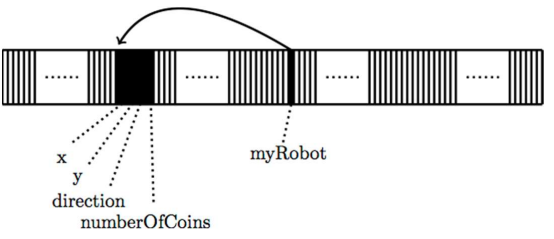
\includegraphics[scale=0.8]{computerspeicher}
	\end{center}

\section{Datenstrukturen}

\begin{tabular}{ | p{0.2\textwidth} p{0.75\textwidth} | }
	\hline
	\makecell[l]{Array} & \makecell[l]{
	$\rhd$ Verwendet zum Speichern von mehreren Variablen des selben Typs \\
	$\rhd$ Erzeugung: \texttt{int[] test = new int[n];} \\
	$\rhd$ \texttt{n} gibt in diesem Fall die feste Anzahl der speicherbaren Variablen an \\
	$\rhd$ Natürlich auch Arrays von Objekten möglich \\
	$\rhd$ Zugriff auf Variablen: \texttt{test[0]} für ersten Wert (Index) \\
	$\rhd$ Zugriff auf Länge: \texttt{test.length} } \\ \hline
	\end{tabular}



\section{Datentypen}

	\begin{tabular}{ | p{0.2\textwidth} p{0.75\textwidth} | }
	\hline

	\makecell[l]{Konstanten} & \makecell[l]{
	$\rhd$ Variable/Referenz wird dadurch unveränderbar \\
	$\rhd$ z.B.: \texttt{final myClass ABC = new myClass();} \\
	\hspace{0.4cm} $\diamond$ Referenz zwar nicht veränderbar, Objekt aber schon \\ 
	$\rhd$ \texttt{Integer.MAX\_VALUE / Integer.MIN\_VALUE} \\
	$\rhd$ Unendlich: \texttt{Double.POSITIVE\_INFINITY / Double.NEGATIVE\_INFINITY} \\
	$\rhd$ Müssen initalisiert werden } \\ \hline
	
	\makecell[l]{Primitive Dateitypen} & \makecell[l]{
	$\rhd$ Ganze Zahlen: byte $\rightarrow$ short $\rightarrow$ int $\rightarrow$ long \\
	$\rhd$ Gebrochene Zahlen: float $\rightarrow$ double \\
	$\rhd$ Logik: boolean \\
	$\rhd$ Zeichen: char \\
	$\rhd$ Mehrere Definitonen: \texttt{int m = 1, n, k = 2;} \\ 
	$\rhd$ Ohne Initialisierung: undefinierter Wert} \\ \hline
	
	\makecell[l]{Literale} & \makecell[l]{
	$\rhd$ wörtlich hingeschriebene Werte eines Datentyps  \\
	$\rhd$ Zahlen standardmä\ss ig int, falls \texttt{long} gewünscht: \texttt{123L oder 123l} \\ 
	$\rhd$ Bei gebrochenen double, falls \texttt{float} gewünscht: \texttt{12.3F oder 12.3f} \\
	$\rhd$ null: Nutzung für Referenzen $\rightarrow$ verweist auf nichts} \\ \hline
	
	\makecell[l]{Boolean} & \makecell[l]{
	$\rhd$ nur \texttt{true} und \texttt{false} \\
	$\rhd$ Negation \texttt{!a} \\
	$\rhd$ Logisches Und: \texttt{a \&\& b} \\
	$\rhd$ Logisches Oder: \texttt{a || b} (inklusiv) \\
	$\rhd$ Gleichheit: \texttt{a == b} } \\ \hline
	
	\makecell[l]{Zeichentyp char} & \makecell[l]{
	$\rhd$ z.B.: \texttt{char c = ´a´;} \\
	$\rhd$ Interne Kodierung als Unicode \\
	$\rhd$ \textbackslash t Horizontaler Tab \\
	$\rhd$ \textbackslash b Backspace \\
	$\rhd$ \textbackslash n Neue Zeile \\
	$\rhd$ Auch Darstellung im Hexacode (\textbackslash u039A)} \\ \hline
	
	\makecell[l]{Enumeration} & \makecell[l]{
	$\rhd$ Zusammenfassung mehrerer Konstanten (feste Anzahl)\\
	$\rhd$ Erzeugung meist in eigener .java Datei \\
	$\rhd$ \texttt{enum MyDirection \{DOWN, RIGHT\} } \\
	$\rhd$ Keine Objekterzeugung von Enumeration möglich \\
	$\rhd$ Abspeichern in Variable des Enum-Types ist jedoch möglich \\
	$\rhd$ \texttt{MyDirection dir = MyDirection.DOWN;} \\
	$\rhd$ Klassenmethoden: \\
	\hspace{0.4cm} $\diamond$ \texttt{values() // Returns array with all enum components} \\
	\hspace{0.4cm} $\diamond$ \texttt{name() // Returns the name of the calling object as string} \\
	 } \\ \hline
	
	\makecell[l]{Referenztypen} & \makecell[l]{
	$\rhd$ Alle Typen, die keine primitiven Datentypen sind \\
	$\rhd$ Unterscheidung zwischen Referez und eigentlichem Objekt \\
	$\rhd$ Gleichheitsoperator \texttt{==} vergleicht nur die Referenz (Objektidentität) \\
	\hspace{0.4cm} $\diamond$ Verweis auf dasselbe Objekt \\
	$\rhd$ Wertgleichheit bezieht sich auf das Objekt an sich \\
	\hspace{0.4cm} $\diamond$ Deep Copy $\Rightarrow$ An allen parallelen Stellen Wertgleichheit \\
	\hspace{0.4cm} $\diamond$ Shallow Copy $\Rightarrow$ Nur Kopie der Adressen \\
	$\rhd$ Ohne Initialisierung: Null} \\ \hline
	\end{tabular}


\section{Exceptions (java.lang.Exception;)}

\begin{tabular}{ | p{0.2\textwidth} p{0.75\textwidth} | }
	\hline
	\makecell[l]{Exception-Klassen} & \makecell[l]{
	$\rhd$ Alle Klassen, die direkt oder indirekt von java.lang.Exception abgeleitet sind} \\ \hline

	\makecell[l]{Exception werfen} & \makecell[l]{
	$\rhd$ \texttt{throws Exception \{...\}} nach Parameterliste im Methodenkopf \\
	$\rhd$ Dies signalisiert, dass die Methode mindestens einen Fehler wirft \\
	$\rhd$ Die geworfene Exception muss vom \texttt{throws}-Typ oder Subtyp sein \\
	$\rhd$ Auch mehrere Exceptions möglich, mit einem Komma getrennt \\
	$\rhd$ Werfen der Exception: \\
	\hspace{0.4cm} $\diamond$ z.B.: \texttt{throw new Exception ("No lower case letter!");} \\
	\hspace{0.4cm} $\diamond$ Hier wird als Parameter für die Objekterstellung ein String übergeben \\
	$\rhd$ \texttt{throws}: \\
	\hspace{0.4cm} $\diamond$ Führt zur Beendung der Methode \\
	\hspace{0.4cm} $\diamond$ Liefert das geworfene Exception-Objekt zurück } \\ \hline

	\makecell[l]{Exception fangen} & \makecell[l]{
	$\rhd$ Bei Methoden, die Exceptions werfen, wird ein \texttt{try-catch}-Block benötigt \\
	$\rhd$ Aufbau: \\
	\hspace{0.4cm} $\diamond$ Methoden, die Exceptions werfen in \texttt{try \{...\}} aufrufen \\
	\hspace{0.4cm} $\diamond$ Falls Exception auftritt wird \texttt{catch (Exception exc) \{...\}} aufgerufen \\
	\hspace{0.4cm} $\diamond$ \texttt{catch} muss direkt im Anschluss nach \texttt{try} stehen \\
	\hspace{0.4cm} $\diamond$ Falls kein Fehler auftritt, wird \texttt{catch} übersprungen \\
	\hspace{0.4cm} $\diamond$ Das Programm wird dann normal weiter ausgeführt \\
	$\rhd$ Es sind auch mehrere \texttt{catch}-Blöcke mit versch. Parametern möglich \\
	$\rhd$ Methoden: \\
	\hspace{0.4cm} $\diamond$ \texttt{getMessage(); // Returns the error message as a string} \\
	\hspace{0.4cm} $\diamond$ \texttt{printStackTrace(); // Ausgabe des Call-Stacks} \\
	$\rhd$ Alle möglichen Exceptions müssen durch den \texttt{catch}-Block abgedeckt sein \\
	$\rhd$ Falls Exception zu mehreren \texttt{catch}-Blöcken 'passt', wird der Erste ausgeführt \\
	\hspace{0.4cm} $\diamond$ Deswegen Reihung der \texttt{catch}-Blöcke von Subtyp nach Supertyp \\
	$\rhd$ Auch mehrere Exceptions in einem \texttt{catch}-Block möglich mit \texttt{||}} \\ \hline

	\makecell[l]{Weiterreichen} & \makecell[l]{
	$\rhd$ Weiterreichen der Fehlermeldung durch \texttt{throws} im Methodenkopf möglich \\
	$\rhd$ Kein \texttt{try-catch}-Block notwendig \\
	$\rhd$ Main-Methode kann z.B. keine Exceptions weiterreichen} \\ \hline

	\makecell[l]{ \texttt{try-with-ressources} } & \makecell[l]{
	$\rhd$ Für Ressourcen, die unbedingt wieder geschlossen werden müssen \\
	$\rhd$ Öffnung der Ressource in runden Klammern: \texttt{try (Printer p =... ) \{...\}} \\
	$\rhd$ Mehrere Ressourcen möglich, getrennt durch Semikolon } \\ \hline

	\makecell[l]{Runtime Exceptions} & \makecell[l]{
	$\rhd$ Ausnahme zu \texttt{try}-Blöcken \\
	$\rhd$ Exceptions von java.lang.RuntimeException und Subtypen \\
	$\rhd$ z.B.: IndexOutOfBoundsException, NullPointerException \\ 
	$\rhd$ Grund: Vermeidung von dauerenden \texttt{try}-Blöcken} \\ \hline
	
	\makecell[l]{Throwable und Error} & \makecell[l]{
	$\rhd$ Exception und Error sind beide von Throwable abgeleitet \\
	$\rhd$ Alle drei befinden sich im Paket java.lang \\
	$\rhd$ Error: \\
	\hspace{0.4cm} $\diamond$ Werden geworfen, falls Fehlerbehandlung keinen Sinn macht \\
	\hspace{0.4cm} $\diamond$ Programmabbruch als Ausweg \\
	$\rhd$ AssertionError: \\
	\hspace{0.4cm} $\diamond$ \texttt{throw new AssertionError("Bad!");} \\
	\hspace{0.4cm} $\diamond$ Kurzform: \texttt{assert x == 2: "Bad!";} \\
	\hspace{0.4cm} $\diamond$ \textbf{Wichtig:} Bedingung muss negiert werden! \\
	\hspace{0.4cm} $\diamond$ Assertanweisungen sinnvoll, da kurz und übersichtlich \\
	\hspace{0.4cm} $\diamond$ Können zusätzlich vom Compiler an- und abgeschaltet werden \\
	\hspace{0.4cm} $\diamond$ z.B.: Verwendung für Tests für Methoden und späteres Abschalten \\
	$\rhd$ Solche Tests werden White-Box-Tests genannt } \\ \hline

	\end{tabular}

\section{Fehler}
	\begin{tabular}{ | p{0.2\textwidth} p{0.75\textwidth} | }
	\hline

	\makecell[l]{Kompilierzeitfehler \\ (compile-time errors)} & \makecell[l]{
	$\rhd$ Falsche Klammersetzung, falsche Schlüsselwörter,..\\
	$\rhd$ Programm wird nicht übersetzt $\Rightarrow$ Fehlermeldung vom Compiler } \\ \hline
	
	\makecell[l]{Laufzeitfehler \\ (run-time errors)} & \makecell[l]{
	$\rhd$ Tritt während der Ausführung auf \\
	$\rhd$ Führt zum Abbruch des Programms $\Rightarrow$ Ausgabe der Fehlermeldung \\
	$\rhd$ Kann nicht vom Compiler entdeckt werden \\
	$\rhd$ IndexOutOfBounds, NullPointerException,.. } \\ \hline
	\end{tabular}

\section{Files}
	\begin{longtable}{ | p{0.2\textwidth} p{0.75\textwidth} | }
	\hline
	
	\makecell[l]{System Properties \\ (java.lang.System)} & \makecell[l]{
	$\rhd$ Attribute der Umgebung, in denen das Java Programm abläuft \\
	$\rhd$ Methoden: \\
	\hspace{0.4cm} $\diamond$ \texttt{getProperty} \\
	\hspace{0.6cm} - Erhält \texttt{String} und gibt \texttt{String} zurück \\ 
	\hspace{0.4cm} $\diamond$ z.B.: \texttt{String homeDir = System.getProperty(\string"user.home\string");} \\
	\hspace{0.4cm} $\diamond$ Mögliche Strings: \\
	\hspace{0.6cm} - \texttt{\string"user.home\string" // Home directory} \\
	\hspace{0.6cm} - \texttt{\string"user.dir\string" // Working directory} \\
	\hspace{0.6cm} - \texttt{\string"user.name\string" // Account name} \\
	\hspace{0.6cm} - \texttt{\string"file.separator\string" // Zeichen zur Dateitrennung} \\
	\hspace{0.6cm} - \texttt{\string"line.separator\string" // Zeichen zur Zeilentrennung} \\
	$\rhd$ \texttt{System.out}: \\
	\hspace{0.4cm} $\diamond$ Klassenattribut \texttt{out} von System ist von Klasse \texttt{PrintStream} \\
	\hspace{0.4cm} $\diamond$ \texttt{PrintStream} hat also auch Methoden wie \texttt{println} \\
	$\rhd$ \texttt{System.err}: \\
	\hspace{0.4cm} $\diamond$ Auch \texttt{err} ist von Klasse \texttt{PrintStream} \\
	\hspace{0.4cm} $\diamond$ Hierhin werden die Fehlerausgaben geschrieben \\
	\hspace{0.4cm} $\diamond$ z.B. sinnvoll um Fehler in seperate Log-Datei umzuleiten \\
	$\rhd$ \texttt{System.in}: \\
	\hspace{0.4cm} $\diamond$ Auch \texttt{in} ist von Klasse \texttt{PrintStream} \\
	\hspace{0.4cm} $\diamond$ Liest Tastatureingaben \\
	$\rhd$ Diese drei Attribute können auch auf andere Streams gesetzt werden \\
	\hspace{0.4cm} $\diamond$ z.B.: andere \texttt{FileInputStreams/FileOutputStreams} \\
	\hspace{0.4cm} $\diamond$ \texttt{System.setIn(in); System.setOut(out); System.setErr(err);}
	} \\ \hline

	\makecell[l]{Klasse Path / Paths} & \makecell[l]{
	$\rhd$ Beide in \texttt{java.nio.file} \\
	$\rhd$ Objekt der Klasse \texttt{Path} verwaltet einen Pfadnamen \\
	\hspace{0.4cm} $\diamond$ Dort muss nicht unbedingt etwas existieren \\
	$\rhd$ \texttt{Paths} wird nur dazu genutzt um Objekt von \texttt{Path} zu erzeugen \\
	\hspace{0.4cm} $\diamond$ z.B.: \texttt{Path path = Paths.get(homeDir, \string"fop.txt\string");}   } \\ \hline

	\makecell[l]{Klasse Files} & \makecell[l]{
	$\rhd$ Aus Package \texttt{java.nio.file} \\
	$\rhd$ Nützliche Sammlung von Klassenmethoden rund um Dateien \\
	$\rhd$ Methoden: \\
	\hspace{0.4cm} $\diamond$ \texttt{lines // Files.lines(path);} \\
	\hspace{0.6cm} - Öffnet Datei an übergebenem Pfad \\
	\hspace{0.6cm} - Liefert einen Stream von Strings, ein String pro Zeile \\
	\hspace{0.6cm} - Zeilenende durch \texttt{\string"file.separator\string"} gekennzeichnet \\
	\hspace{0.6cm} - \texttt{IOException}, falls Problem beim Öffnen der Datei (\texttt{java.io}) \\
	\hspace{0.4cm} $\diamond$ \texttt{exists // Files.exists(path);} \\
	\hspace{0.6cm} - \texttt{true}, wenn es dort Datei/Verzeichnis gibt \\
	\hspace{0.4cm} $\diamond$ \texttt{isReadable(path)} \\
	\hspace{0.6cm} - Fragt lesende Zugriffsrechte ab \\
	\hspace{0.4cm} $\diamond$ \texttt{isWritable(path)} \\
	\hspace{0.6cm} - Fragt schreibende Zugriffsrechte ab \\
	\hspace{0.4cm} $\diamond$ \texttt{isRegularFile(path)} \\
	\hspace{0.6cm} - \texttt{true}, falls es eine reguläre Datei ist (kein Verzeichnis) \\
	\hspace{0.4cm} $\diamond$ \texttt{isDirectory(path)} \\
	\hspace{0.6cm} - \texttt{true}, falls es ein Verzeichnis ist \\
	\hspace{0.4cm} $\diamond$ \texttt{size(path) // long size = Files.size(path);} \\
	\hspace{0.6cm} - Fragt die Grö\ss e der Datei ab \\
	\hspace{0.6cm} - \texttt{long}, da die Dateigröe oft nicht in \texttt{int} passt \\
	\hspace{0.4cm} $\diamond$ \texttt{createFile(path)} \\
	\hspace{0.6cm} - Richtet Datei an der übergebenen Stelle ein \\
	\hspace{0.4cm} $\diamond$ \texttt{copy(path1, path2)} \\
	\hspace{0.6cm} - Kopieren von Pfad 1 nach Pfad 2 \\
	\hspace{0.4cm} $\diamond$ \texttt{move(path1, path2)} \\
	\hspace{0.6cm} - Umbenennen einer Datei, oft auch Bewegen genannt \\
	\hspace{0.4cm} $\diamond$ \texttt{delete(path)} \\
	\hspace{0.6cm} - Entfernen einer Datei \\
	\hspace{0.6cm} - \texttt{NoSuchElementException}, falls nicht vorhanden \\
	\hspace{0.4cm} $\diamond$ \texttt{deleteIfExists(path)} \\
	\hspace{0.6cm} - Falls das Objekt nicht existiert, passiert garnichts} \\ \hline
	
	\makecell[l]{Beispiel: \\ Einlesen einer Datei \\  in einen String} & \makecell[l]{
	1 \hspace{0.1cm} \texttt{String homeDir = System.getProperty(\string"user.home\string");} \\
	2 \hspace{0.1cm} \texttt{Path path = Paths.get(homeDir, \string"fop\string", \string"streams.txt\string");} \\
	3 \hspace{0.1cm} \texttt{try (Stream<String> stream = Files.lines(path)) \{ }  \\
	4 \hspace{0.5cm} \texttt{String fileContentAsString = stream.reduce(String::concat);} \\
	5 \hspace{0.1cm} \texttt{\} catch (IOException exc) \{ } \\
	6 \hspace{0.5cm} \texttt{System.out.print(\string"Could not open file\string")} \\
	7 \hspace{0.1cm} \texttt{\}} \\
	$\rhd$ \texttt{try-with-resources} wird für Interface \texttt{AutoCloseable} verwendet } \\ \hline

	\makecell[l]{Bytedaten} & \makecell[l]{
	$\rhd$ Direkt, ohne Bezug zu Streams \\
	$\rhd$ Klassen und Interfaces finden sich in \texttt{java.io} \\
	$\rhd$ Byteweise Verarbeitung sinnvoll für Audio oder Bilddateien, nicht für Text \\
	$\rhd$ Wird aber meist durch Bibliotheken oder Ähnliches gehandhabt} \\ \hline

	\makecell[l]{Bytedaten lesen} & \makecell[l]{
	$\rhd$ Verwendung eines \texttt{InputStream}-Objekts \\
	$\rhd$ \texttt{InputStream} abstrakt, deswegen nur Subtypen z.B.: \texttt{FileInputStream} \\
	\hspace{0.4cm} $\diamond$ \texttt{FileInputStream} nutzt den Namen der Datei als String im Konstruktor \\
	$\rhd$ Methoden: \\
	\hspace{0.4cm} $\diamond$ \texttt{read()} \\
	\hspace{0.6cm} - Liest nächstes Byte in ein \texttt{int} \\
	\hspace{0.6cm} - Überprüfung, ob -1 um zu prüfen, ob Dateiende erreicht ist \\
	$\rhd$ Beispiel: \\
	\hspace{0.4cm} 1 \hspace{0.1cm} \texttt{FileInputStream in = new FileInputStream (fileName);} \\
	\hspace{0.4cm} 2 \hspace{0.1cm} \texttt{int n = in.read();} \\
	\hspace{0.4cm} 3 \hspace{0.1cm} \texttt{if (n == 1) return;} } \\ \hline

	\makecell[l]{Bytedaten schreiben} & \makecell[l]{
	$\rhd$ Verwendung eines \texttt{OutputStream}-Objekts \\
	$\rhd$ \texttt{OutputStream} abstrakt, deswegen nur Subtypen z.B.: \texttt{FileOutputStream} \\
	\hspace{0.4cm} $\diamond$ \texttt{FileOutputStream} nutzt den Namen der Datei als String im Konstruktor \\
	\hspace{0.4cm} $\diamond$ Existiert die Datei schon, geht der Inhalt verloren \\
	\hspace{0.4cm} $\diamond$ Existiert die Datei nicht, wird sie erstellt \\
	\hspace{0.4cm} $\diamond$ Zweiter Konstruktor mit \texttt{boolean} als zweiten Paramter: \\
	\hspace{0.6cm} - Falls \texttt{false}: Verhält sich wie normaler Konstruktor \\
	\hspace{0.6cm} - Falls \texttt{true}: Inhalt geht nicht verloren, wird hinten angehangen  \\
	$\rhd$ Methoden: \\
	\hspace{0.4cm} $\diamond$ \texttt{write()} \\
	\hspace{0.4cm} $\diamond$ Hat \texttt{int} als formalen Parametertyp \\
	\hspace{0.4cm} $\diamond$ Schreibt nur unterestes Byte dieses \texttt{int} \\
	$\rhd$ Beispiel: \\
	\hspace{0.4cm} 1 \hspace{0.1cm} \texttt{FileOutputStream out = new FileOutputStream(fileName);} \\  
	\hspace{0.4cm} 2 \hspace{0.1cm} \texttt{int i = 5;} \\
	\hspace{0.4cm} 3 \hspace{0.1cm} \texttt{out.write(i);}} \\ \hline

	\makecell[l]{Relevante Subtypen  von \\Input-/OutputStream} & \makecell[l]{
	$\rhd$ Geschwindigkeit beim Lesen/Schreiben ist relevant \\
	$\rhd$ \texttt{BufferedInputStream}: \\
	\hspace{0.4cm} $\diamond$ liest mehrere Bytes auf einmal ein \\
	\hspace{0.4cm} $\diamond$ Konstruktor: \texttt{BufferedInputStream(InputStream in)} \\
	\hspace{0.4cm} $\diamond$ Verwendet im Konstruktor z.B. einen \texttt{FileInputStream} \\
	$\rhd$ \texttt{BufferedOutputStream}: \\
	\hspace{0.4cm} $\diamond$ Schreibt zuerst in internen Puffer \\
	\hspace{0.4cm} $\diamond$ Falls dieser voll ist, wird in die Datei geschrieben \\
	\hspace{0.4cm} $\diamond$ Konstruktor: \texttt{BufferedOutputStream(OutputStream out)} \\
	\hspace{0.4cm} $\diamond$ Schreibt die Daten auf den OutputStream im Parameter \\
	$\rhd$ \texttt{PrintStream}: \\
	\hspace{0.4cm} $\diamond$ Ersatz für OutputStream im Package \texttt{java.io} \\
	\hspace{0.4cm} $\diamond$ Konstruktor: \texttt{PrintStream(OutputStream out)} \\
	\hspace{0.4cm} $\diamond$ Dient als Konvertierer von primitiven Datentypen und String \\
	\hspace{0.8cm} in die byteweise Darstellung \\
	\hspace{0.4cm} $\diamond$ Das eigentliche Schreiben übernimmt der übergebene \texttt{OutputStream} \\
	\hspace{0.4cm} $\diamond$ Methode \texttt{print} \\ 
	\hspace{0.6cm} - z.B.: \texttt{out1.print("pi = "); out1.print(3.14);} \\
	\hspace{0.6cm} - Byteweise Ausgabe von übergebenen Werten \\
	\hspace{0.4cm} $\diamond$ \texttt{System.out.print()}: \texttt{out} ist von Klasse \texttt{PrintStream} \\
	\hspace{0.4cm} $\diamond$ Methode \texttt{println} \\
	\hspace{0.6cm} - Ausgabe von Werten mit Zeilenumbruch} \\ \hline

	\makecell[l]{Mehr Subtypen von \\Input-/OutputStream} & \makecell[l]{
	$\rhd$ \texttt{java.util.zip.ZipInputStream} \\
	\hspace{0.4cm} $\diamond$ Zum Einlesen von komprimierten Zip-Dateien \\
	$\rhd$ \texttt{java.util.jar.JarInputStream} \\
	\hspace{0.4cm} $\diamond$ Zum Einlesen von Jar-Dateien \\
	\hspace{0.4cm} $\diamond$ Jar-Dateien enthalten kompilierte Java-Dateien, mit zip komprimiert \\
	$\rhd$ \texttt{javax.sound.sampled.AudioInputStream} \\
	\hspace{0.4cm} $\diamond$ für Audio-Dateien \\
	$\rhd$ \texttt{java.io.PipedInputStream / java.io.PipedOutputStream} \\
	\hspace{0.4cm} $\diamond$ Zwei aneinander gekoppelte Lese/Schreib-Klassen
	} \\ \hline

	\makecell[l]{Textdaten direkt} & \makecell[l]{
	$\rhd$ Bequemere Zugriffsmöglichkeiten für Textdaten vorhanden \\
	$\rhd$ \texttt{Reader} und \texttt{Writer} aus Package \texttt{java.io} \\
	$\rhd$ Textdatei besteht aus einzelnen Zeichen aka \texttt{char} \\
	\hspace{0.4cm} $\diamond$ Jedes \texttt{char} ist zwei Byte gro\ss} \\ \hline

	\makecell[l]{Textdaten lesen} & \makecell[l]{
	$\rhd$ Komplett analog zu \texttt{InputStream} und \texttt{FileInputStream} \\
	$\rhd$ \texttt{Reader} abstrakt, deswegen nur Subtypen z.B. \texttt{FileReader} \\
	\hspace{0.4cm} $\diamond$ \texttt{FileReader} nutzt den Namen der Datei als String im Konstruktor \\
	$\rhd$ Methoden: \\
	\hspace{0.4cm} $\diamond$ \texttt{read} \\
	\hspace{0.6cm} - Liest \texttt{char}-Werte ein \\
	\hspace{0.6cm} - Verschiedene Implementationen z.B.: kein Parameter $\rightarrow$ einzelner \texttt{char} \\
	\hspace{0.6cm} - Mit \texttt{char-Array}: Liest soviele ein, bis \texttt{Array} voll ist \\
	$\rhd$ Beispiel: \\
	\hspace{0.4cm} 1 \hspace{0.1cm} \texttt{FileReader reader1 = new FileReader(fileName);} \\
	\hspace{0.4cm} 2 \hspace{0.1cm} \texttt{char[] buffer = new char[256];} \\
	\hspace{0.4cm} 3 \hspace{0.1cm} \texttt{int n = reader1.read(buffer);} \\
	\hspace{0.4cm} 4 \hspace{0.1cm} \texttt{// n ist in diesem Fall die Anzahl der gelesenen chars} \\
	$\rhd$ \texttt{BufferedReader} \\
	\hspace{0.4cm} $\diamond$ Konstruktor: \texttt{BufferedReader(Reader in)} \\
	\hspace{0.4cm} $\diamond$ Methode \texttt{readLine();} \\
	\hspace{0.6cm} - Liest alles vom letzten gelesenen Zeichen bis zum Zeilenende \\
	\hspace{0.6cm} - Also meist eine ganze Zeile \\
	$\rhd$ Verknüpfung mit byteweisem Einlesen: \\
	\hspace{0.4cm} $\diamond$ evtl. sinnvoll, falls offener \texttt{InputStream} auf Text-Datenquelle \\
	\hspace{0.4cm} $\diamond$ Die Brücke bildet hier der Subtyp \texttt{InputStreamReader} \\
	\hspace{0.4cm} 1 \hspace{0.1cm} \texttt{InputStream in = ...;} \\
	\hspace{0.4cm} 2 \hspace{0.1cm} \texttt{Reader reader = new InputStreamReader(in);}} \\ \hline

	\makecell[l]{Textdaten schreiben} & \makecell[l]{
	$\rhd$ \texttt{Writer} abstrakt, deswegen nur Subtypen z.B. \texttt{FileWriter} \\
	\hspace{0.4cm} $\diamond$ \texttt{FileWriter} benutzt den Namen der Datei als String im Konstruktor \\
	$\rhd$ Methoden: \\
	\hspace{0.4cm} $\diamond$ \texttt{write} \\
	\hspace{0.6cm} - Schreibt einzelnen \texttt{char} oder ganzen \texttt{String} \\
	$\rhd$ Beispiel: \\
	\hspace{0.4cm} 1 \hspace{0.1cm} \texttt{FileWriter writer1 = new FileWriter(fileName);} \\
	\hspace{0.4cm} 2 \hspace{0.1cm} \texttt{writer1.write('H');} \\
	\hspace{0.4cm} 3 \hspace{0.1cm} \texttt{writer1.write(\string"ello World\string");} \\ 
	$\rhd$ Verknüpfung mit byteweisem Schreiben: \\
	\hspace{0.4cm} $\diamond$ Die Brücke bildet hier der Subtyp \texttt{OutputStreamWriter} \\
	\hspace{0.4cm} 1 \hspace{0.1cm} \texttt{OutputStream out = ...;} \\
	\hspace{0.4cm} 2 \hspace{0.1cm} \texttt{Writer writer = new OutputStreamWriter(out);} } \\ \hline

	\end{longtable}


\section{Graphical User Interface}
	\begin{longtable}{ | p{0.2\textwidth} p{0.75\textwidth} | }
	\hline
	
	\makecell[l]{Window Manager} & \makecell[l]{
	$\rhd$ Systemprozess, der permanent im Hintergrund als \texttt{Service} läuft \\
	$\rhd$ Stellt generelle, anwendungsunspezifische Funktionalitäten zur Verfügung \\
	\hspace{0.4cm} $\diamond$ Öffnen, Schlie\ss en, Ikonifizieren, Grö\ss e ändern \\
	\hspace{0.4cm} $\diamond$ Rahmen um Fenster, Bildschirmhintergrund } \\ \hline

	\makecell[l]{Klasse Frame} & \makecell[l]{
	$\rhd$ Abgeleitet von \texttt{java.awt.Window;} (awt = abstract window toolkit) \\
	$\rhd$ Im Gegensatz zu \texttt{Window} aber mit Rahmen (vom \texttt{Window Manager} verwaltet) \\
	$\rhd$ Beispielkonstruktor: \texttt{Frame frame = new Frame(string); // Fenstertitel} \\
	$\rhd$ Vorhergehensweise: \\
	\hspace{0.4cm} $\diamond$ Erstellung einer Klasse, die \texttt{Frame} erweitert \\
	\hspace{0.4cm} $\diamond$ Hinzufügen von Funktionalitäten \\
	$\rhd$ Methoden: \\
	\hspace{0.4cm} $\diamond$ \texttt{setVisible(boolean b)} \\ 
	\hspace{0.6cm} - \texttt{Frame} ist entweder sichtbar oder unsichtbar \\ 
	\hspace{0.6cm} - Standardmä\ss ig unsichtbar \\
	\hspace{0.6cm} - Erst Fenster aufbauen, dann sichtbar machen \\
	\hspace{0.4cm} $\diamond$ \texttt{setBackground(Color bgColor)} \\
	\hspace{0.6cm} - Setzt die Hintergrundfarbe des Fensters \\
	\hspace{0.4cm} $\diamond$ \texttt{dispose()} \\
	\hspace{0.6cm} - Alle Ressourcen des Fensters und der Bestandteile werden freigegeben \\
	\hspace{0.4cm} $\diamond$ \texttt{setExtendedState(int state)} \\
	\hspace{0.6cm} - Setzt den Status des Fensters \\
	\hspace{0.6cm} - \texttt{ICONIFIED}: Ikonifiziert das Fenster \\
	\hspace{0.6cm} - \texttt{NORMAL}: Deikonifiziert das Fenster \\
	\hspace{0.6cm} - \texttt{MAXIMIZED\_HORIZ}: Ausbreitung auf gesamte Horizontale \\
	\hspace{0.4cm} $\diamond$ \texttt{add(Component comp)} \\
	\hspace{0.6cm} - Fügt den übergebenen Komponenten zum \texttt{Frame} hinzu \\
	} \\ \hline

	\makecell[l]{Komponenten} & \makecell[l]{
	$\rhd$ Eigene Klasse für jede Komponente \\
	$\rhd$ Alle Klassen oder Interfaces aus \texttt{java.awt}, falls nicht anders gesagt \\
	$\rhd$ Werden mithilfe von \texttt{add(Component comp)} zum Fenster hinzugefügt } \\ \hline

	\makecell[l]{Button} & \makecell[l]{$\rhd$ Konstruktor: \texttt{Button(String label) // Text auf dem Button} \\
	$\rhd$ Methoden: \\
	\hspace{0.4cm} $\diamond$ \texttt{setFont(Font f)} \\
	\hspace{0.6cm} - Zum Setzen der Schriftart \\
	\hspace{0.6cm} - Konstruktor \texttt{Font: Font(String name, int style, int size)} \\
	\hspace{0.4cm} $\diamond$ \texttt{addActionListener(ActionListener l)} \\
	\hspace{0.6cm} - Fügt den übergebenen \texttt{ActionListener} hinzu \\ 
	\hspace{0.6cm} - Bei jedem Klick wird \texttt{actionPerformed} des \texttt{Listeners} aufgerufen \\
	\hspace{0.6cm} - Auch mehrere möglich \\
	\hspace{0.6cm} - Automatische Einrichtung des \texttt{Event Dispatch Thread} \\
	\hspace{0.4cm} $\diamond$ \texttt{setLabel(String label)} \\
	\hspace{0.6cm} - Setzt den Titel des \texttt{Button}
	} \\ \hline

	\makecell[l]{Interface ActionListener} & \makecell[l]{
	$\rhd$ Zugehörig zu \texttt{Button} \\
	$\rhd$ Aus Package \texttt{java.awt.event} \\
	$\rhd$ Funktionales Interface \\
	$\rhd$ Funktionale Methode \texttt{actionPerformed (ActionEvent event)} \\
	$\rhd$ Vorhergehensweise: \\
	\hspace{0.4cm} $\diamond$ Erstellen einer eigenen Klasse, die \texttt{ActionListener} implementiert \\
	\hspace{0.4cm} $\diamond$ Erstellen relevanter Attribute und Konstruktor für gegebenen Fall \\
	\hspace{0.4cm} $\diamond$ Implemetieren der Methode \texttt{actionPerformed (ActionEvent event)} \\
	\hspace{0.4cm} $\diamond$ Erstellen eines Objekts unserer Klasse \\ 
	\hspace{0.6cm} - \texttt{ActionListener listener = new MyListener(frame);} \\
	\hspace{0.4cm} $\diamond$ Hinzufügen des \texttt{Listener} zum \texttt{Button} \\
	\hspace{0.6cm} - \texttt{button.addActionListener(listener);} \\
	$\rhd$ Alternativ: \\
	\hspace{0.4cm} $\diamond$ Erstellung des \texttt{Listener} in der Subklasse des \texttt{Frame} \\ 
	\hspace{0.6cm} - Keine \texttt{Frame}-Übergabe notwendig \\
	\hspace{0.6cm} - z.B.: als \texttt{private}-Klasse (Stichwort: \texttt{nested classes}) \\
	 } \\ \hline

	\makecell[l]{Klasse ActionEvent} & \makecell[l]{
	$\rhd$ Übergebener Parameter bei \texttt{actionPerformed} \\
	$\rhd$ Methoden: \\
	\hspace{0.4cm} $\diamond$ \texttt{getWhen()} \\
	\hspace{0.6cm} - Gibt die Uhrzeit des Geschehnisses als \texttt{long} zurück \\
	\hspace{0.6cm} - Nützlich: \texttt{java.sql.Timestamp} \\
	\hspace{0.6cm} - \texttt{Timestamp stamp = new Timestamp (event.getWhen());} \\ 
	\hspace{0.6cm} - Methoden: \texttt{stamp.getHour(); stamp.getMinute();}} \\ \hline

	\makecell[l]{Übersicht Listener und \\ Events} & \makecell[l]{
	$\rhd$ \texttt{Listener}-Interface $\leftrightarrow$ \texttt{Event}-Klasse \\
	$\rhd$ \texttt{KeyListener} $\leftrightarrow$ \texttt{KeyEvent} \\
	$\rhd$ \texttt{MouseListener} $\leftrightarrow$ \texttt{MouseEvent} \\
	$\rhd$ \texttt{MouseMotionListener} $\leftrightarrow$ \texttt{MouseEvent} \\
	$\rhd$ \texttt{MouseWheelListener} $\leftrightarrow$ \texttt{MouseWheelEvent} \\ 
	$\rhd$ \texttt{WindowFocusListener} $\leftrightarrow$ \texttt{WindowEvent} \\
	$\rhd$ \texttt{WindowListener} $\leftrightarrow$ \texttt{WindowEvent} \\ 
	$\rhd$ \texttt{WindowStateListener} $\leftrightarrow$ \texttt{WindowEvent} \\
	$\rhd$ Hinzufügen: \\
	\hspace{0.4cm} $\diamond$ \texttt{addKeyListener(...)} \\
	\hspace{0.4cm} $\diamond$ \texttt{addMouseListener(...)} \\
	\hspace{0.4cm} $\diamond$ \texttt{addWindowListener(...)} } \\ \hline

	\makecell[l]{Adapter} & \makecell[l]{
	$\rhd$ Verwendung von Adaptern, wenn passendes Interface nicht \texttt{functional} ist \\
	\hspace{0.4cm} $\diamond$ z.B. Interface \texttt{KeyListener, MouseListener,..} \\
	\hspace{0.4cm} $\diamond$ Diese Interfaces besitzen mehrere Methoden \\
	$\rhd$ Adapter sind Klassen und bestehen zu jedem \texttt{Listener}-Interface \\
	\hspace{0.4cm} $\diamond$ z.B.: \texttt{KeyAdapter, MouseAdapter} \\
	\hspace{0.4cm} $\diamond$ Diese Adapter implementieren das dazugehörige Interface \\
	\hspace{0.4cm} $\diamond$ Die Methoden werden jedoch leer gelassen \\
	$\rhd$ Vorteil vom Adapter: \\
	\hspace{0.4cm} $\diamond$ Nicht alle Methoden müssen implementiert werden \\
	\hspace{0.4cm} $\diamond$ Nur die genutzten Methoden (z.B.: \texttt{keyPressed()}) werden implementiert \\
	$\rhd$ Verwendung: \\
	\hspace{0.4cm} $\diamond$ Erweitern der eigenen \texttt{Listener}-Klasse mit Adapter \\
	\hspace{0.4cm} $\diamond$ z.B.: \texttt{public class MyKeyListener extends KeyAdapter \{...\}}} \\ \hline

	\makecell[l]{Interface KeyListener} & \makecell[l]{
	$\rhd$ Abhorchen der Tastatur \\
	$\rhd$ Erstellen eigener Klasse, die die Klasse \texttt{KeyAdapter} (siehe Adapter) erweitert \\
	$\rhd$ Methoden: \\
	\hspace{0.4cm} $\diamond$ \texttt{public void keyPressed (KeyEvent event)} \\
	\hspace{0.6cm} - Wird beim Herunterdrücken einer Taste ausgeführt \\
	\hspace{0.4cm} $\diamond$ \texttt{public void keyReleased (KeyEvent event)} \\
	\hspace{0.6cm} - Wird beim Loslassen einer Taste ausgeführt \\
	\hspace{0.4cm} $\diamond$ \texttt{public void keyTyped (KeyEvent event)} \\
	\hspace{0.6cm} - Wird beim Antippen einer Taste ausgeführt} \\ \hline

	\makecell[l]{Klasse KeyEvent} & \makecell[l]{
	$\rhd$ Übergebener Parameter bei z.B.: \texttt{keyPressed} \\
	$\rhd$ Methoden: \\
	\hspace{0.4cm} $\diamond$ \texttt{getKeyCode()} \\
	\hspace{0.6cm} - Liefert die Kodierung der gedrückten Taste zurück \\
	$\rhd$ Klassenkonstanten für jede Taste: \\
	\hspace{0.4cm} $\diamond$ z.B.: \texttt{KeyEvent.VK\_A // Buchstabe A} \\
	\hspace{0.4cm} $\diamond$ z.B.: \texttt{KeyEvent.VK\_COLON // Doppelpunkt} \\
	\hspace{0.4cm} $\diamond$ z.B.: \texttt{KeyEvent.VK\_BACKSPACE // Backspace Taste} \\
	$\rhd$ Beispiel Verwendung: \\
	\hspace{0.4cm} 1 \hspace{0.1cm} \texttt{public class MyKeyListener extends KeyAdapter \{} \\
	\hspace{0.4cm} 2 \hspace{0.5cm} \texttt{public void keyPressed (KeyEvent event) \{} \\
	\hspace{0.4cm} 3 \hspace{0.9cm} \texttt{switch (event.getKeyCode()) \{}	\\
	\hspace{0.4cm} 4 \hspace{1.3cm} \texttt{case KeyEvent.VK\_A: ... break;} \\
	\hspace{0.4cm} 5 \hspace{1.3cm} \texttt{case KeyEvent.VK\_COLON: ... break;} \\
	\hspace{0.4cm} 6 \hspace{1.3cm} \texttt{case KeyEvent.VK\_Backspace: ... break;} \\
	\hspace{0.4cm} 7 \hspace{0.9cm} \texttt{\}} \\
	\hspace{0.4cm} 8 \hspace{0.5cm} \texttt{\}} \\
	\hspace{0.4cm} 9 \hspace{0.1cm} \texttt{\}}
	} \\ \hline

	\makecell[l]{Interface MouseListener} & \makecell[l]{
	$\rhd$ Abhorchen der Maus \\
	$\rhd$ Erstellen eigener Klasse, die die Klasse \texttt{MouseAdapter} erweitert \\
	\hspace{0.4cm} $\diamond$ \texttt{MouseAdapter} implementiert alle drei \texttt{Mouse}-Interfaces \\
	\hspace{0.4cm} $\diamond$  \texttt{MouseListener, MouseMotionListener, MouseWheelListener} \\
	$\rhd$ Methoden: \\
	\hspace{0.4cm} $\diamond$ \texttt{public void mouseClicked (MouseEvent event)} \\
	\hspace{0.6cm} - Wird beim kurzen Klicken der Maustaste ausgeführt \\
	\hspace{0.4cm} $\diamond$ \texttt{public void mousePressed (MouseEvent event)} \\	
	\hspace{0.6cm} - Wird beim Herunterdrücken der Maustaste ausgeführt \\
	\hspace{0.4cm} $\diamond$ \texttt{public void mouseReleased (MouseEvent event)} \\
	\hspace{0.6cm} - Wird beim Loslassen der Maustaste ausgeführt \\
	\hspace{0.4cm} $\diamond$ \texttt{public void mouseEntered (MouseEvent event)} \\
	\hspace{0.6cm} - Wird ausgeführt, sobald der Mauszeiger den abgehorchten Bereich betritt \\
	\hspace{0.4cm} $\diamond$ \texttt{public void mouseExited (MouseEvent event)} \\
	\hspace{0.6cm} - Wird ausgeführt, sobald der Mauszeiger den abgehorchten Bereich verlässt} \\ \hline

	\makecell[l]{Interface \\ MouseMotionListener} & \makecell[l]{
	$\rhd$ Abhorchen der Mausbewegung \\
	$\rhd$ Methoden sind auch in Klasse \texttt{MouseAdapter} enthalten \\
	$\rhd$ Methoden: \\
	\hspace{0.4cm} $\diamond$ \texttt{public void mouseDragged (MouseEvent event)} \\
	\hspace{0.4cm} $\diamond$ \texttt{public void mouseMoved (MouseEvent event)}  } \\ \hline

	\makecell[l]{Interface \\ MouseWheelListener} & \makecell[l]{
	$\rhd$ Abhorchen der Mausradbewegung \\
	$\rhd$ Methoden sind auch in Klasse \texttt{MouseAdapter} enthalten \\
	$\rhd$ Methoden: \\
	\hspace{0.4cm} $\diamond$ \texttt{public void mouseWheelMoved (MouseWheelEvent event)}} \\ \hline

	\makecell[l]{Klasse MouseEvent} & \makecell[l]{
	$\rhd$ Übergebener Parameter bei z.B.: \texttt{mouseClicked} \\
	$\rhd$ Methoden: \\
	\hspace{0.4cm} $\diamond$ \texttt{getButton()} \\
	\hspace{0.6cm} - Liefert die gedrückte Taste zurück \\
	\hspace{0.4cm} $\diamond$ \texttt{getX()} \\
	\hspace{0.6cm} - Liefert x-Koordinate abhängig vom Ursprung des Bereichs \\
	\hspace{0.4cm} $\diamond$ \texttt{getY()} \\
	\hspace{0.6cm} - Liefert y-Koordinate abhängig vom Ursprung des Bereichs \\
	$\rhd$ Klassenkonstanten für Maustasten: \\
	\hspace{0.4cm} $\diamond$ \texttt{MouseEvent.BUTTON1} \\
	\hspace{0.4cm} $\diamond$ \texttt{MouseEvent.BUTTON2}} \\ \hline

	\makecell[l]{Klasse \\ MouseWheelEvent} & \makecell[l]{
	$\rhd$ Übergebener Parameter bei z.B.: \texttt{mouseWheelMoved} \\
	$\rhd$ Methoden: \\
	\hspace{0.4cm} $\diamond$ \texttt{getWheelRotation()} \\
	\hspace{0.6cm} - Liefert die Anzahl der gedrehten "Ticks"  } \\ \hline

	\makecell[l]{Interface \\ WindowListener} & \makecell[l]{
	$\rhd$ Abhorchen von Fensteraktionen \\
	$\rhd$ Erstellen eigener Klasse, die die Klasse \texttt{WindowAdapter} erweitert \\
	\hspace{0.4cm} $\diamond$ \texttt{WindowAdapter} implementiert alle drei \texttt{Window}-Interfaces \\
	\hspace{0.4cm} $\diamond$ \texttt{WindowListener, WindowStateListener, WindowFocusListener} \\
	$\rhd$ Methoden: \\
	\hspace{0.4cm} $\diamond$ \texttt{public void windowOpened (WindowEvent event)} \\
	\hspace{0.4cm} $\diamond$ \texttt{public void windowClosing (WindowEvent event)} \\
	\hspace{0.4cm} $\diamond$ \texttt{public void windowClosed (WindowEvent event)} \\
	\hspace{0.4cm} $\diamond$ \texttt{public void windowClosed (WindowEvent event)} \\
	\hspace{0.4cm} $\diamond$ \texttt{public void windowDeactivated (WindowEvent event)} \\
	\hspace{0.4cm} $\diamond$ \texttt{public void windowIconified (WindowEvent event)} \\
	\hspace{0.4cm} $\diamond$ \texttt{public void windowDeiconified (WindowEvent event)}} \\ \hline

	\makecell[l]{Interface \\ WindowStateListener} & \makecell[l]{
	$\rhd$ Abhorchen des Status des Fensters \\
	$\rhd$ Methoden sind auch in \texttt{WindowAdapter} vorhanden \\
	$\rhd$ Methoden: \\
	\hspace{0.4cm} $\diamond$ \texttt{public void windowStateChanged ( WindowEvent event )}} \\ \hline

	\makecell[l]{Interface \\ WindowFocusListener} & \makecell[l]{
	$\rhd$ Abhorchen des Fokus im Bezug auf das Fenster \\
	$\rhd$ Methoden sind auch in \texttt{WindowAdapter} vorhanden \\
	$\rhd$ Methoden: \\
	\hspace{0.4cm} $\diamond$ \texttt{public void windowGainedFocus ( WindowEvent event )} \\
	\hspace{0.4cm} $\diamond$ \texttt{public void windowLostFocus ( WindowEvent event )} } \\ \hline

	\makecell[l]{Klasse Canvas} & \makecell[l]{
	$\rhd$ abgegrenzte Zeichenfläche in einem Fenster \\
	$\rhd$ Vorhergehensweise: \\
	\hspace{0.4cm} $\diamond$ Erstellung eigener Subtyp-Klasse von \texttt{Canvas} \\
	\hspace{0.4cm} $\diamond$ Implementieren der Methode \texttt{public void paint (Graphics graphics)} \\
	\hspace{0.4cm} $\diamond$ Füllen der Methode mit eigener Zeichenlogik \\
	\hspace{0.4cm} $\diamond$ Verwendung von \texttt{java.awt.Graphics;} \\
	\hspace{0.4cm} $\diamond$ Hinzufügen zum \texttt{Frame} mithilfe von \texttt{add} \\
	$\rhd$ Beleuchtung nützlicher Aspekte von Graphics: \\
	$\rhd$ \texttt{FontMetrics} \\
	\hspace{0.4cm} $\diamond$ Informationen über festgelegte Schriftart und Schriftgröße \\
	\hspace{0.4cm} $\diamond$ Abfrage: \\
	\hspace{0.6cm} - \texttt{FontMetrics fontM = graphics.getFontMetrics();} \\
	\hspace{0.4cm} $\diamond$ Abfrage der maximalen Stringhöhe: \\
	\hspace{0.6cm} - \texttt{int maxHeight = fontM.getMaxAscent() + fontM.getMaxDescent();} \\
	\hspace{0.6cm} - Methoden geben maximalen Abstand von der Basislinie des Textes an \\
	\hspace{0.4cm} $\diamond$ Abfrage der Stringbreite von gegebenem String: \\
	\hspace{0.6cm} - \texttt{int widthStr = fontMetrics.stringWidth(string);} \\
	$\rhd$ Abfrage des Zeichenfensters als Rechteck: \\
	\hspace{0.6cm} - \texttt{Rectangle area = graphics.getClipBounds();} \\
	\hspace{0.6cm} - \texttt{x} und \texttt{y} geben den Ursprung an \\
	\hspace{0.6cm} - \texttt{width} und \texttt{height} die Breite und Höhe \\
	$\rhd$ Einige Methoden von \texttt{Graphics} \\
	\hspace{0.4cm} $\diamond$ \texttt{setColor(Color color)} \\
	\hspace{0.4cm} $\diamond$ \texttt{fillOval(...)} \\
	\hspace{0.4cm} $\diamond$ \texttt{drawOval(...)} \\
	\hspace{0.4cm} $\diamond$ \texttt{drawString(...)}} \\ \hline

	\makecell[l]{Klasse Checkbox} & \makecell[l]{
	$\rhd$ Kleiner Button (Pin) mit etwas Text \\
	$\rhd$ Zwei Zustände: An oder Aus \\
	$\rhd$ Konstruktor: \\
	\hspace{0.4cm} $\diamond$ \texttt{Checkbox(String label) // Titel der Checkbox} \\
	\hspace{0.4cm} $\diamond$ \texttt{Checkbox} standardmä\ss ig aus \\
	$\rhd$ Benötigt ein Objekt vom Typ \texttt{ItemListener} (siehe unten) \\
	\hspace{0.4cm} $\diamond$ \texttt{ItemListener item = new MyItemListener(checkbox,...);} \\
	$\rhd$ Methoden: \\
	\hspace{0.4cm} $\diamond$ \texttt{isSelected()} \\
	\hspace{0.6cm} - \texttt{true}, wenn die \texttt{Checkbox} an ist \\
	\hspace{0.4cm} $\diamond$ \texttt{setLabel(string);} \\
	\hspace{0.6cm} - Setzt den Titel der \texttt{Checkbox}} \\ \hline

	\makecell[l]{Interface \\ ItemListener} & \makecell[l]{
	$\rhd$ Verwendung bei \texttt{Checkbox} und \texttt{Choice} \\
	$\rhd$ Funktionales Interface \\
	$\rhd$ Funktionale Methode \texttt{itemStateChanged (ItemEvent event)} \\
	$\rhd$ Vorhergehensweise analog zu \texttt{ActionListener} \\
	\hspace{0.4cm} $\diamond$ Erstellung neuer Klasse, die \texttt{ItemListener} implementiert} \\ \hline

	\makecell[l]{Klasse Choice} & \makecell[l]{
	$\rhd$ Repräsentiert ein Auswahlmenü \\
	$\rhd$ Verwendet auch das Interface \texttt{ItemListener} \\
	$\rhd$ Konstruktor: \\
	\hspace{0.4cm} $\diamond$ \texttt{Choice choice = new Choice();}
	$\rhd$ Methoden: \\
	\hspace{0.4cm} $\diamond$ \texttt{add(string)} \\
	\hspace{0.6cm} - Hinzufügen neuer Auswahlen \\
	\hspace{0.6cm} - Startet bei Index 0 \\
	\hspace{0.4cm} $\diamond$ \texttt{select(int)} \\
	\hspace{0.6cm} - Legt eine Auswahl als Standard fest \\
	\hspace{0.6cm} - Übergabe des Index als \texttt{int}
	\hspace{0.4cm} $\diamond$ \texttt{getSelectedItem()} \\
	\hspace{0.6cm} - Liefert den ausgewählten String zurück \\
	\hspace{0.4cm} $\diamond$ \texttt{getSelectedIndex()} \\
	\hspace{0.6cm} - Liefert Index der aktiven Auswahl } \\ \hline

	\makecell[l]{Klasse Label} & \makecell[l]{
	$\rhd$ Nicht durch User interagierbares Rechteck mit Text \\
	$\rhd$ Konstruktor: \\
	\hspace{0.4cm} $\diamond$ \texttt{Label(String text) // Labeltext} \\
	$\rhd$ Wartet auf Events bei anderen Entitäten \\
	$\rhd$ Methoden: \\
	\hspace{0.4cm} $\diamond$ \texttt{setAlignment(int alignment)} \\
	\hspace{0.6cm} - Auswahl der Zentierung des Textes \\
	\hspace{0.6cm} - Paramter: \texttt{Label.CENTER, Label.RIGHT, Label.LEFT} \\
	\hspace{0.4cm} $\diamond$ \texttt{setBackground(Color c)} \\
	\hspace{0.6cm} - Setzen der Hintergrundfarbe \\
	\hspace{0.4cm} $\diamond$ \texttt{	setText(String text)} \\
	\hspace{0.6cm} - Setzt den Text des \texttt{Label} \\
	\hspace{0.6cm} - z.B.: Aufruf beim Drücken eines \texttt{Button}} \\ \hline

	\makecell[l]{Klasse List} & \makecell[l]{
	$\rhd$ Auswahlmenü \\
	$\rhd$ Aus \texttt{java.awt}, \textbf{nicht} \texttt{java.util} \\
	$\rhd$ Konstruktor:  \\
	\hspace{0.4cm} $\diamond$ \texttt{List(int rows, boolean multipleMode)} \\
	\hspace{0.4cm} $\diamond$ \texttt{rows} gibt die maximale Anzahl der zugleich angezeigten Menüpunkte an \\
	\hspace{0.4cm} $\diamond$ Anzahl der Möglichkeiten größer als \texttt{rows} $\rightarrow$ Scrollbar \\
	\hspace{0.4cm} $\diamond$ \texttt{multipleMode}: Auswahl mehrerer Menüpunkte ermöglichen \\
	$\rhd$ Methoden: \\
	\hspace{0.4cm} $\diamond$ \texttt{add(String item)} \\
	\hspace{0.6cm} - Hinzufügen neuer Menüpunkte \\
	\hspace{0.4cm} $\diamond$ \texttt{getSelectedIndexes()} \\
	\hspace{0.6cm} - Liefert die Indizes der ausgewählten Punkte \\
	\hspace{0.4cm} $\diamond$ \texttt{setMultipleMode(boolean b)} \\
	\hspace{0.6cm} - De-/Aktivieren der Mehrfachauswahl} \\ \hline

	\makecell[l]{Klasse Scrollbar} & \makecell[l]{
	$\rhd$ Werden meist automatisch hinzugefügt (\texttt{List}) \\
	$\rhd$ z.B.: Erstellung eines eigenen Schiebereglers \\
	$\rhd$ Benötigt ein Objekt vom Typ \texttt{AdjustmentListener} (siehe unten) \\
	\hspace{0.4cm} $\diamond$ z.B.: \texttt{AdjustmentListener adjust = new MyAdjustListener(frame);} \\
	$\rhd$ Konstruktor: \\
	\hspace{0.4cm} $\diamond$ \texttt{Scrollbar(int orientation, int value, int visible,} \\
	\hspace{2.5cm} \texttt{ int minimum, int maximum)} \\
	\hspace{0.4cm} $\diamond$ \texttt{orientation}: \texttt{Scrollbar.VERTICAL, Scrollbar.HORIZONTAL} \\
	\hspace{0.4cm} $\diamond$ \texttt{value}: Startwert der Scrollbar \\
	\hspace{0.4cm} $\diamond$ \texttt{visible}: Grö\ss e des scrollbaren Balkens \\
	\hspace{0.4cm} $\diamond$ \texttt{minimum}: Minimal einstellbarer Wert \\
	\hspace{0.4cm} $\diamond$ \texttt{maximum}: Maximal einstellbarer Wert} \\ \hline

	\makecell[l]{Interface \\ AdjustmentListener} & \makecell[l]{
	$\rhd$ Verwendung bei \texttt{Scrollbar} \\
	$\rhd$ Funktionales Interface \\
	$\rhd$ Funktionale Methode: \texttt{adjustmentValueChanged (AdjustmentEvent event)} \\
	$\rhd$ Vorhergehensweise analog zu \texttt{ActionListener} \\
	\hspace{0.4cm} $\diamond$ Erstellung neuer Klasse, die \texttt{AdjustmentListener} implementiert} \\ \hline

	\makecell[l]{Klasse \\ Adjustmentevent} & \makecell[l]{$\rhd$ Übergebener Parameter bei \texttt{adjustmentValueChanged} \\
	$\rhd$ Methoden: \\
	\hspace{0.4cm} $\diamond$ \texttt{getValue()} \\
	\hspace{0.6cm} - Liefert den neuen Wert der Scrollbar} \\ \hline

	\makecell[l]{Klasse Textfield} & \makecell[l]{
	$\rhd$ Zeile, vom Nutzer schreibbar \\
	$\rhd$ z.B.: Benutzername, Passwort, etc.. \\
	$\rhd$ Benötigt ein Objekt vom Typ \texttt{KeyListener} (siehe oben) \\
	$\rhd$ Konstruktor: \\
	\hspace{0.4cm} $\diamond$ \texttt{TextField(int columns)} \\
	\hspace{0.4cm} $\diamond$ \texttt{columns} gibt die Zeichenzahl in der Zeile an \\
	$\rhd$ Methoden: \\
	\hspace{0.4cm} $\diamond$ \texttt{setEchoChar(char c)} \\
	\hspace{0.6cm} - Anzeige der eingegebenen Zeichen mit anderem Zeichen z.B.: '*' \\
	\hspace{0.6cm} - Rückgängig machen: \texttt{field.setEchochar((char) 0);} \\
	$\rhd$ Methoden: \\
	\hspace{0.4cm} $\diamond$ \texttt{getText()} \\
	\hspace{0.6cm} - Liefert den eingegebenen Text als String} \\ \hline

	\makecell[l]{Klasse TextArea} & \makecell[l]{
	$\rhd$ Eingabebereich über mehrere Zeilen \\
	$\rhd$ z.B.: Verwendung eines Objekts des Typs \texttt{FocusListener} \\
	$\rhd$ Konstruktor: \\
	\hspace{0.4cm} $\diamond$ \texttt{TextArea(String text, int rows, int columns, int scrollbars)} \\
	\hspace{0.4cm} $\diamond$ \texttt{text}: Text, falls Bereich leer und nicht im Mausfokus \\
	\hspace{0.4cm} $\diamond$ \texttt{scrollbars}: Legt die Art der \texttt{Scrollbar} fest \\
	\hspace{0.6cm} - \texttt{Scrollbar.BOTH, Scrollbar.HORIZONTAL\_ONLY} \\
	\hspace{0.6cm} - \texttt{Scrollbar.NONE, Scrollbar.VERTICAL\_ONLY} \\
	\hspace{0.4cm} $\diamond$ \texttt{rows}: Anzahl der Zeilen \\
	\hspace{0.4cm} $\diamond$ \texttt{columns}: Breite der Zeilen \\
	$\rhd$ Methoden: \\
	\hspace{0.4cm} $\diamond$ \texttt{setText(String t)} \\
	\hspace{0.6cm} - Setzt den Text des Textfeldes \\
	\hspace{0.4cm} $\diamond$ \texttt{getText()} \\
	\hspace{0.6cm} - Liefert den geschriebenen Text als String \\
	$\rhd$ Leerer Text: \texttt{(\string"\string")} \\
	\hspace{0.4cm} $\diamond$ z.B.: Vergleich mit momentanem Text mit \texttt{equals}} \\ \hline

	\makecell[l]{Interface FocusListener} & \makecell[l]{
	$\rhd$ Verwendung bei \texttt{TextArea} \\
	$\rhd$ Kein funktionales Interface, trotzdem keine Adapter-Klasse \\
	$\rhd$ Vorhergehensweise analog zu \texttt{ActionListener} \\
	$\rhd$ Im Gegensatz zu \texttt{WindowFocusListener} auch für einzelne Komponenten \\
	$\rhd$ Methoden: \\
	\hspace{0.4cm} $\diamond$ \texttt{focusGained(FocusEvent e)} \\ 
	\hspace{0.6cm} - Wird ausgeführt, wenn eine Komponente den Tastaturfokus erhält \\
	\hspace{0.4cm} $\diamond$ \texttt{focusLost(FocusEvent e)} \\
	\hspace{0.6cm} - Wird ausgeführt, wenn eine Komponente den Tastaturfokus verliert} \\ \hline

	\makecell[l]{Hierarchie graphischer \\ Komponenten} & \makecell[l]{
	$\rhd$ Vom \texttt{java.awt.Component} direkt abgeleitet: \\
	\hspace{0.4cm} $\diamond$ \texttt{Button} \\
	\hspace{0.4cm} $\diamond$ \texttt{Canvas} \\
	\hspace{0.4cm} $\diamond$ \texttt{Checkbox} \\
	\hspace{0.4cm} $\diamond$ \texttt{Choice} \\
	\hspace{0.4cm} $\diamond$ \texttt{Label} \\
	\hspace{0.4cm} $\diamond$ \texttt{List} \\
	\hspace{0.4cm} $\diamond$ \texttt{Scrollbar} \\
	\hspace{0.4cm} $\diamond$ \texttt{TextComponent // Supertyp von TextArea und TextField} \\
	\hspace{0.4cm} $\diamond$ \texttt{Container}
	$\rhd$ Von \texttt{Container} direkt abgeleitet: \\
	\hspace{0.4cm} $\diamond$ \texttt{Window} \\
	$\rhd$ Von \texttt{Window} direkt abgeleitet: \\
	\hspace{0.4cm} $\diamond$ \texttt{Frame} } \\ \hline


	\makecell[l]{Klasse Component} & \makecell[l]{
	$\rhd$ Die meisten Methoden sind hier definiert, aber nicht implementiert \\
	\hspace{0.4cm} $\diamond$ z.B.: \texttt{setVisible(boolean b), setFont(Font f),..} \\
	\hspace{0.4cm} $\diamond$ Die Methoden werden in den Komponentenklassen dann implementiert} \\ \hline

	\makecell[l]{Klasse Container} & \makecell[l]{
	$\rhd$ Fasst mehrere Komponenten zu einer zusammen \\
	$\rhd$ Hinzufügen von \texttt{Buttons,..., Windows, Frames, Containern} möglich \\
	$\rhd$ \textbf{Wichtig:} Hinzufügen von \texttt{Container} möglich \\
	\hspace{0.4cm} $\diamond$ Ähnliche Struktur wie ein Ordnerverzeichnis \\
	\hspace{0.4cm} $\diamond$ z.B.: \texttt{Frame} in einem \texttt{Frame} \\
	$\rhd$ Methoden: \\
	\hspace{0.4cm} $\diamond$ \texttt{paint (Graphics graphics)} \\
	\hspace{0.6cm} - In \texttt{Component} definiert, hier überschrieben \\
	\hspace{0.6cm} - Ruft \texttt{paint} für jeden enthaltenen Komponenten auf \\
	\hspace{0.4cm} $\diamond$ \texttt{add (Component comp)} \\
	\hspace{0.6cm} - Hinzufügen einer Komponente zum \texttt{Container} \\
	\hspace{0.4cm} $\diamond$ \texttt{add (Component comp, Object constraints)} \\
	\hspace{0.6cm} - Steuerung der Position mithilfe des zweiten Parameters \\ \\
	\hspace{0.6cm} - Weiteres bei \texttt{LayoutManager} \\
	\hspace{0.4cm} $\diamond$ \texttt{setLayout (LayoutManager manager)} \\
	\hspace{0.6cm} - Setzen des \texttt{LayoutManager} \\
	\hspace{0.6cm} - Dieser steuert die Platzierung der Komponenten \\ 
	\hspace{0.6cm} - Jeder \texttt{Container} hat zu jedem Zeitpunkt einen \texttt{LayoutManager} \\
	\hspace{0.4cm} $\diamond$ \texttt{validate()} \\
	\hspace{0.6cm} - Aktualisierung nach z.B.: Grö\ss enänderung } \\ \hline

	\makecell[l]{Klasse LayoutManager} & \makecell[l]{
	$\rhd$ Wird bei Erstellung eines \texttt{Containers} oder Subtyps automatisch eingerichtet \\
	\hspace{0.4cm} $\diamond$ Standardklasse für für \texttt{Window} und \texttt{Frame} ist \texttt{BorderLayout} \\
	$\rhd$ \texttt{BorderLayout} \\
	$\rhd$ Einteilung des Fensters in fünf Bereiche \\
	\hspace{0.4cm} $\diamond$ \texttt{NORTH, EAST, SOUTH, WEST, CENTER} \\
	\hspace{0.4cm} $\diamond$ Mögliche Positionen als Klassenkonstaten vordefiniert \\
	\hspace{0.6cm} - z.B.: \texttt{BorderLayout.NORTH, BorderLayout.CENTER,..} \\
	\hspace{0.4cm} $\diamond$ Verwendung bei \texttt{add (Component comp, Object constraints)} \\
	\hspace{0.6cm} - z.B.: \texttt{frame.add (comp1, BorderLayout.NORTH);} \\
	\hspace{0.6cm} - Ohne Wahl der Position (normales \texttt{add}): \texttt{CENTER} als Standard \\
	$\rhd$ \texttt{BorderLayout} an sich für das Fenster an sich meist die richtige Wahl \\
	\hspace{0.4cm} $\diamond$ Aber nicht unbedingt für \texttt{Container} innerhalb eines Fensters \\
	$\rhd$ \texttt{BoxLayout} \\ 
	\hspace{0.4cm} $\diamond$ Anlegen in einer Reihe nacheinander \\
	\hspace{0.4cm} $\diamond$ Wahl ob vertikal oder horizontal im Konstruktor \\
	$\rhd$ \texttt{GridLayout} \\
	\hspace{0.4cm} $\diamond$ Matrixartiges Anlegen (wie Telefontastatur) \\
	\hspace{0.4cm} $\diamond$ Anzahl Zeilen und Spalten im Konstruktor festgelegt \\
	$\rhd$ \texttt{BorderLayout, BoxLayout und GridLayout}: \\
	\hspace{0.4cm} $\diamond$ Passen Größe der Komponenten anhand der Gesamtsituation an \\
	\hspace{0.4cm} $\diamond$ Nicht unbedingt passendste Größe für Komponente \\
	$\rhd$ \texttt{FlowLayout} \\
	\hspace{0.4cm} $\diamond$ Anlegen in einer Zeile nebeneinander \\
	\hspace{0.6cm} - Anfangen einer Zeile, falls die alte voll ist \\
	\hspace{0.4cm} $\diamond$ Wählt automatisch die bestmöglichste Größe für Komponenten \\
	\hspace{0.6cm} - Abfrage über \texttt{getPreferredSize()} \\
	$\rhd$ \texttt{CardLayout} \\
	\hspace{0.4cm} $\diamond$ Zeigt Komponenten nicht alle gleichzeitig, sondern nacheinander \\
	\hspace{0.4cm} $\diamond$ Navigation: \texttt{first, last, next, previous} \\
	$\rhd$ \texttt{validate()} \\
	\hspace{0.4cm} $\diamond$ Notwendig zur Aktualisierung von sichtbaren Fenstern \\
	\hspace{0.4cm} $\diamond$ Wann: \\
	\hspace{0.6cm} - Ändern der Anzahl von Komponenten \\
	\hspace{0.6cm} - Ändern der Grö\ss e von Komponenten (auch Schrift)} \\ \hline

	\makecell[l]{Java Swing (javax.swing)} & \makecell[l]{
	$\rhd$ \texttt{java.awt} als Grundlage \\
	$\rhd$ Zweite Bibliothek, die die Funktionalitäten erweitert \\
	$\rhd$ Verbindung zu \texttt{java.awt}: \\
	\hspace{0.4cm} $\diamond$ \texttt{JFrame extends java.awt.Frame} \\
	\hspace{0.4cm} $\diamond$ \texttt{JComponent extends java.awt.Container} \\
	\hspace{0.6cm} - Funktionalitäten von \texttt{Container} hier in \texttt{JComponent} \\
	$\rhd$ Von \texttt{JComponent} abgeleitet: \\
	\hspace{0.4cm} $\diamond$ \texttt{JButton, JCheckbox, JLabel} \\
	\hspace{0.4cm} $\diamond$ \texttt{JList<T>, JScrollbar, JTextComponent} \\
	$\rhd$ \texttt{JButton, JCheckbox} sind aber indirekt abgeleitet: \\
	\hspace{0.4cm} $\diamond$ Zwischenklasse \texttt{AbstractButton} bei beiden \\
	\hspace{0.6cm} - \texttt{public class JButton extends AbstractButton\{\}} \\
	\hspace{0.4cm} $\diamond$ Bei \texttt{JCheckbox} zusätzlich noch \texttt{JToggleButton extends AbstractButton} \\
	\hspace{0.6cm} - \texttt{public class JCheckbox extends JToggleButton \{\}} \\
	\hspace{0.4cm} $\diamond$ \textbf{Grund:} \\
	\hspace{0.6cm} - Einführung zusätzlicher, eng verwandter, Komponenten \\
	\hspace{0.6cm} - Deswegen Auslagerung in Supertyp \\
	$\rhd$ \texttt{JList<T>}: \\
	\hspace{0.4cm} $\diamond$ in \texttt{Swing} generisch, Liste von beliebigem Referenztyp \\
	\hspace{0.4cm} $\diamond$ in \texttt{java.awt} wird String verwendet} \\ \hline
	 
	\makecell[l]{Klasse JComponent} & \makecell[l]{
	$\rhd$ Bietet mehr Funktionalitäten als \texttt{Component} \\
	$\rhd$ ToolTips: \\
	\hspace{0.4cm} $\diamond$ Hinzufügen von MouseOver-ToolTips \\
	\hspace{0.4cm} $\diamond$ \texttt{setToolTipText(String s)} \\
	\hspace{0.6cm} - Setzen des Tooltip-Texts \\
	\hspace{0.4cm} $\diamond$ Deaktivieren mithilfe Übergabe von \texttt{null} \\
	$\rhd$ \texttt{Randdarstellungen:} \\
	\hspace{0.4cm} $\diamond$ Ränder für Komponenten \textbf{innerhalb} eines Fensters \\
	\hspace{0.4cm} $\diamond$ \texttt{setBorder (Border border)} \\
	\hspace{0.4cm} $\diamond$ Verwendung der Klasse \texttt{BorderFactory} zur Erzeugung der \texttt{Border} \\
	\hspace{0.6cm} - \texttt{BorderFactory.createLineBorder(Color color,int thickness)} \\
	\hspace{0.8cm} - Simpler rechteckiger Rahmen mit angegebener Dicke und Farbe \\
	\hspace{0.6cm} - \texttt{BorderFactory.createBevelBorder(BevelBorder.LOWERED)} \\
	\hspace{0.6cm} - \texttt{BorderFactory.createBevelBorder(BevelBorder.RAISED)} \\
	\hspace{0.8cm} - Ganze Komponente mit 3D Effekt (tiefer oder höher erscheinend) \\
	\hspace{0.6cm} - \texttt{BorderFactory.createEtchedBorder(EtchedBorder.LOWERED)} \\
	\hspace{0.6cm} - \texttt{BorderFactory.createEtchedBorder(EtchedBorder.RAISED)} \\
	\hspace{0.8cm} - Nur Rand mit 3D Effekt (tiefer oder höher erscheinend) \\
	\hspace{0.6cm} - \texttt{BorderFactory.createEmptyBorder()} \\
	\hspace{0.8cm} - Zurücksetzen des Randeffekts \\
	$\rhd$ \texttt{Look and Feel:} \\
	\hspace{0.4cm} $\diamond$ Anpassung der Gesamterscheinung an Systemstandard \\
	\hspace{0.4cm} $\diamond$ Verwendung von \texttt{javax.swing.UIManager} \\
	\hspace{0.4cm} $\diamond$ Setzen des Look and Feel auf Systemstandard: \\
	\hspace{0.8cm} 1 \hspace{0.1cm} \texttt{String s = UIManager.getSystemLookAndFeelClassName();}  \\
	\hspace{0.8cm} 2 \hspace{0.1cm} \texttt{UIManager.setLookAndFeel(s);} \\
	\hspace{0.4cm} $\diamond$ Setzen des Look and Feel auf z.B. Java-Standard \\
	\hspace{0.8cm} Methode: \texttt{UIManager.setLookAndFeel(LookAndFeel lookAndFeel)} \\
	\hspace{0.8cm} 1 \hspace{0.1cm} \texttt{UIManager.setLookAndFeel(new MetalLookAndFeel());}  \\
	$\rhd$ \texttt{KeyBindings:} \\
	\hspace{0.4cm} $\diamond$ Funktionalitäten wie \texttt{Listener} automatisch umgesetzt \\
	\hspace{0.4cm} $\diamond$ Erläuterung der Funktion anhand eines Beispiels: \\
	\hspace{0.8cm} 1 \hspace{0.1cm} \texttt{String keyStrokeStr = \string"alt shift X\string";} \\
    \hspace{0.8cm} 2 \hspace{0.1cm} \texttt{KeyStroke keystroke = KeyStroke.getKeyStroke(keyStrokeStr);} \\
    \hspace{0.8cm} 3 \hspace{0.1cm} \texttt{textArea.getInputMap().put(keystroke, keyStrokeStr);} \\
	\hspace{0.8cm} 4 \hspace{0.1cm} \texttt{StyledEditorKit.UnderlineAction action } \\
	\hspace{0.8cm} 5 \hspace{0.5cm} \texttt{= new StyledEditorkit.UnderlineAction();} \\
	\hspace{0.8cm} 6 \hspace{0.1cm} \texttt{textArea.getActionMap().put(keyStrokeStr, action);} \\
	\hspace{0.6cm} - Zeile 1: Kodierung einer Tastenkombination als String \\
	\hspace{0.6cm} - Regeln dafür: Dokumentation \texttt{javax.swing.KeyStroke} \\
	\hspace{0.6cm} - Zeile 2: Umwandlung des Strings in \texttt{KeyStroke}-Objekt \\
	\hspace{0.6cm} - Jeder \texttt{JComponent} hat \texttt{actionMap} und \texttt{inputMap} (ähnlich wie \texttt{Map}) \\
	\hspace{0.6cm} - Zeile 3 und 6: Einfügen von \texttt{Key + Value} in jeweilige \texttt{Map} \\
	\hspace{0.6cm} - Verbindung dieser \texttt{Maps} über \texttt{Value} von Input und \texttt{Key} von Action \\
	\hspace{0.6cm} - Verbindung über \texttt{keyStrokeStr} einer Aktion mit Tastenkombination \\
	\hspace{0.6cm} - Zeile 4 und 5: Verwendung von \texttt{Action extends ActionListener} \\
	\hspace{0.6cm} - Verwendung der Methode \texttt{actionPerformed} \\
	\hspace{0.6cm} - Klassen in Java vorhanden, die \texttt{Action} implementieren (UnderlineAction) \\
	\hspace{0.6cm} - Klasse \texttt{UnderlineAction} ist in Klasse \texttt{StyledEditorKit} eingebettet \\
	\hspace{0.6cm} - Enthält viele Funktionalitäten zum Editieren von Texten \\
	$\rhd$ \texttt{Drag \& Drop:} \\
	\hspace{0.4cm} $\diamond$ Automatisch implementiert, Konfiguration möglich \\
	$\rhd$ \texttt{Assistive Technologies:} \\
	\hspace{0.4cm} $\diamond$ Unterstützungsmöglichkeiten für Leute mit Handicap \\
	$\rhd$ Zusätzliche Features von \texttt{JFrame}: \\
	\hspace{0.4cm} $\diamond$ Separierung von Hauptmenü und Rest des Fensters} \\ \hline
	
	\makecell[l]{Weitere GUI-Klassen} & \makecell[l]{
	$\rhd$ \texttt{JFormattedTextfield}: \\
	\hspace{0.4cm} $\diamond$ Erlaubt Formatierungsregeln für den einzugebenden Text \\
	\hspace{0.4cm} $\diamond$ z.B. für Datumsangaben
	\hspace{0.4cm} $\diamond$ \texttt{JFormattedTextField extends JTextField} \\
	$\rhd$ \texttt{JPasswordField}: \\
	\hspace{0.4cm} $\diamond$ Zusätzliche Funktionalitäten für Passwörter \\
	$\rhd$ \texttt{JRadioButton}: \\
	\hspace{0.4cm} $\diamond$ kleiner, anklickbarer Bereich \\
	\hspace{0.4cm} $\diamond$ Verwendung im Rahmen eines Objekts von Klasse \texttt{ButtonGroup} \\
	\hspace{0.4cm} $\diamond$ Nur ein \texttt{RadioButton} in \texttt{ButtonGroup} kann gleichzeitig angeklickt sein \\
	$\rhd$ \texttt{JToolbar}: \\
	\hspace{0.4cm} $\diamond$ Vereinfachte Möglichkeit für Standardmenüs \\
	$\rhd$ \texttt{JSlider}: \\
	\hspace{0.4cm} $\diamond$ Klasse für Schieberegler \\
	\hspace{0.4cm} $\diamond$ Besser als Verwendung einer \texttt{Scrollbar} als Schieberegler \\
	$\rhd$ \texttt{Popup}: \\
	\hspace{0.4cm} $\diamond$ Popup-Fenster \\
	$\rhd$ \texttt{JTable}: \\
	\hspace{0.4cm} $\diamond$ Umsetzung einer Tabelle \\
	\hspace{0.4cm} $\diamond$ Häufiges Verwendungsbeispiel: \\
	\hspace{0.8cm} 1 \hspace{0.1cm} \texttt{Object[][] entries = ...;} \\
	\hspace{0.8cm} 2 \hspace{0.1cm} \texttt{Object[] columnNames = ...;} \\
	\hspace{0.8cm} 3 \hspace{0.1cm} \texttt{JTable table = new JTable(entries, columnNames);} \\
	\hspace{0.8cm} 4 \hspace{0.1cm} \texttt{JScrollPane scrollPane = new JScrollPane(table);} \\
	\hspace{0.8cm} 5 \hspace{0.1cm} \texttt{table.setFillsViewportHeight(true);} \\
	\hspace{0.8cm} 6 \hspace{0.1cm} \texttt{int[] selectedRows = table.getSelectedRows();} \\
	\hspace{0.8cm} 7 \hspace{0.1cm} \texttt{int[] selectedColumns = table.getSelectedColumns();} \\
	\hspace{0.6cm} - Zeile 1: Erzeugung der Tabellenmatrix \\
	\hspace{0.6cm} - Zeile 2: Erzeugung der Spaltennamen \\
	\hspace{0.6cm} - Zeile 3: Konstruktor der Tabelle mit den eben erstellen Arrays \\
	\hspace{0.6cm} - Zeile 4: \texttt{JScrollPane} kapselt Objekt von \texttt{Component} ein \\
	\hspace{0.6cm} - Zeigt nur einen Ausschnitt der übergebenen Komponente \\
	\hspace{0.6cm} - Fügt au\ss erdem \texttt{Scrollbar} ein \\
	\hspace{0.6cm} - Zeile 5: Vertikale Streckung der Tabelle, um gesamte Höhe auszufüllen \\
	\hspace{0.6cm} - Zeile 6: Abfrage der momentan ausgewählten Zeile \\
	\hspace{0.6cm} - Zeile 7: Abfrage der momentan ausgewählten Spalte} \\ \hline
	
	
	
	\end{longtable}





\section{Generics}
	\begin{longtable}{ | p{0.2\textwidth} p{0.75\textwidth} | }
	\hline
	\makecell[l]{Wrapper-Klassen} & \makecell[l]{
	$\rhd$ primitive Datentypen nicht mit Generizität vereinbar \\
	$\rhd$ Deswegen benötigen wir eine stellvertretende Klasse $\rightarrow$ Wrapper-Klassen \\
	$\rhd$ selber Name, nur mit gro"sem Anfangsbuchstaben (Integer, Long, Character,..) \\
	$\rhd$ Konstruktor mit Parameter des zugehörigen Datentyps \\
	$\rhd$ Methoden: \\
	\hspace{0.4cm} $\diamond$ \texttt{intValue(); // Returns specific value of class} \\
	\hspace{0.4cm} $\diamond$ \texttt{MAX\_VALUE; // Returns max value} \\
	$\rhd$ Boxing/Unboxing: \\
	\hspace{0.4cm} $\diamond$ Primitiver Datentyp und Wrapper-Klasse sind austauschbar \\
	\hspace{0.4cm} $\diamond$ Automatische Umwandlung ineinander \\
	\hspace{0.4cm} $\diamond$ Boxing: \texttt{Integer i = 123;} \\
	\hspace{0.4cm} $\diamond$ Unboxing: \texttt{System.out.print(i); // 123} } \\ \hline
	
	\makecell[l]{Generische Klassen} & \makecell[l]{
	$\rhd$ \texttt{public class Pair <T1, T2> \{...\}} \\
	$\rhd$ Klasse \texttt{Pair} ist \textbf{generisch} / Klasse \texttt{Pair} ist mit T1 und T2 \textbf{parametrisiert} \\
	$\rhd$ \texttt{T1} und \texttt{T2} sind die \textbf{Typparameter} von Klasse \texttt{Pair} \\
	$\rhd$ \texttt{T1} und \texttt{T2} können als Datentypen/Rückgabewerte verwendet werden \\
	$\rhd$ Können \textbf{nicht} in Klassenmethoden verwendet werden  \\
	$\rhd$ Bei Einrichtung von Objekten von \texttt{Pair} werden die Typparamter festgelegt \\
	\hspace{0.4cm} $\diamond$ \texttt{Pair<Integer,Double> pair = new Pair<Integer,Double>(2,3.5);} \\
	\hspace{0.4cm} $\diamond$ \texttt{Pair} ist mit \texttt{Integer} und \texttt{Double} \textbf{instanziiert}\\
	\hspace{0.4cm} $\diamond$ Typparameter können natürlich auch vom selben Typ sein} \\ \hline

	\makecell[l]{Generische Methoden} & \makecell[l]{
	$\rhd$ Auch in \textbf{nicht-generischen Klassen} generische Methoden möglich \\
	$\rhd$ \texttt{public class X \{...\}} \\
	$\rhd$ Einzelne Methode parametrisiert: \\
	\hspace{0.4cm} $\diamond$ \texttt{public <T1,T2> Pair<T1,T2> makePair(T1 t1, T2 t2) \{...\}} \\
	\hspace{0.4cm} $\diamond$ \textbf{Parametrisierung} der Methode (\texttt{<T1,T2>}) steht vor dem Rückgabetyp \\
	$\rhd$ Aufurf: \\
	\hspace{0.4cm} $\diamond$ \texttt{Pair<A,B> pair1 = x.makePair(new A(), new B());} \\
	\hspace{0.4cm} $\diamond$ Compiler erkennt selbst die Typen für die Methode \\
	$\rhd$ Falls \texttt{T1} z.B. schon die Klasse \texttt{X} parametrisiert: \\
	\hspace{0.8cm} \texttt{public class X <T1>} \{ \\
	\hspace{1.2cm} \texttt{public <T2> Pair<T1,T2> makePair(T1 t1, T2 t2) \{...\} } \\
	\hspace{0.8cm} \} } \\ \hline 

	\makecell[l]{Typparameter} & \makecell[l]{
	$\rhd$ Alle Arten von Klassen und Arrays möglich \\
	$\rhd$ Auch parametrisierte Klassen sind als Typparamter möglich \\
	$\rhd$ Typparameter dürfen jedoch nicht vom primitiven Datentyp sein \\
	$\rhd$ Vererbung von Typparametern ist jedoch nicht übertragbar \\ 
	\hspace{0.4cm} $\diamond$ Bei bereits instanziierten Parametern sind keine Subklassen möglich \\
	$\rhd$ Kurzform: \\
	\hspace{0.4cm} $\diamond$ \texttt{Pair<String,Integer> pair;} \\
	\hspace{0.4cm} $\diamond$ \texttt{pair = new Pair<> ("Hello", 123);} \\
	\hspace{0.4cm} $\diamond$ \texttt{"Diamond-Operator"}: Compiler erkennt selbstständig die Instanziierung } \\ \hline

	\makecell[l]{Eingeschränkte \\ Typparameter} & \makecell[l]{
	$\rhd$ Werden bei der Definition von generischen Klassen/Methoden verwendet \\
	$\rhd$ \texttt{<T extends X> // T gleich X, oder direkt/indirekt Subtyp von X} \\
	\hspace{0.4cm} $\diamond$ Notwendig um sicherzustellen, dass aufgerufene Methoden definiert sind \\
	\hspace{0.4cm} $\diamond$ z.B.: \texttt{<T extends Number> // z.B.: doubleValue() immer vorhanden} \\
	$\rhd$ Mehrfache Einschränkung:  \\
	\hspace{0.4cm} $\diamond$ \texttt{<T extends X \& Interface1 \& Interface2} \\
	\hspace{0.4cm} $\diamond$ Klasse muss, falls vorhanden, an erster Stelle stehen} \\ \hline

	\makecell[l]{Wildcards} & \makecell[l]{
	$\rhd$ Werden bei der Instanziierung von Typparametern verwendet \\
	$\rhd$ \texttt{public double m (X<? extends Number> n) \{...\}} \\
	\hspace{0.4cm} $\diamond$ Ermöglicht nun die Verwendung von Subklassen bei aktualen Parametern \\
	\hspace{0.4cm} $\diamond$ (Siehe Einschränkung \texttt{Typparameter / 4. Stichpunkt}) \\
	$\rhd$ \textbf{Unterschied:} \\
	\hspace{0.4cm} $\diamond$ \texttt{public <T extends Number> double m (X<T> n) \{...\}} \\
	\hspace{0.6cm} $\diamond$ Generische Methode mit eingeschränkt wählbarem Typparameter \\
	\hspace{0.4cm} $\diamond$ \texttt{public double m (X<? extends Number> n) \{...\}} \\
	\hspace{0.6cm} $\diamond$ Nichtgenerische Methode mit generischem Parameter mit eingeschränkt \\
	\hspace{1cm} wählbarem Typparameter \\
	$\rhd$ Weitere Wildcard: \texttt{X<?>} \\
	\hspace{0.4cm} $\diamond$ Allgemeinst möglichste, \texttt{extends Object} \\
	$\rhd$ \texttt{X<? super Double>} \\
	\hspace{0.4cm} $\diamond$ Mit allen Supertypen (direkt/indirekt) und alle implementieren Interfaces} \\ \hline

	\makecell[l]{Empfehlungen} & \makecell[l]{
	$\rhd$ Oracle-Empfehlungen im Bezug auf Wildcards \\
	$\rhd$ In-Parameter (Werte einer Methode, die nur gelesen werden): \\ 
	\hspace{0.4cm} $\diamond$ Verwendung von \texttt{extends} \\
	$\rhd$ Out-Paramter (Werte einer Methode, die nur geschrieben werden): \\
	\hspace{0.4cm} $\diamond$ Verwendung von \texttt{super} \\
	$\rhd$ In/Out-Parameter: \\
	\hspace{0.4cm} $\diamond$ Keine Verwendung von Wildcards \\
	$\rhd$ Rückgaben: \\
	\hspace{0.4cm} $\diamond$ Keine Verwendung von Wildcards} \\ \hline

	\makecell[l]{Interface Comparator} & \makecell[l]{
	$\rhd$  \texttt{Functional Interface} im Package \texttt{java.util} \\
	$\rhd$ Verwendung: \\
	\hspace{0.4cm} $\diamond$ Erstellen einer Vergleichsklasse, die \texttt{Comparator<T>} implementiert \\
	\hspace{0.4cm} $\diamond$ \texttt{..class MyComp<T extends Number> implements Comparator<T> \{...\}} \\
	\hspace{0.4cm} $\diamond$ Generisch mit einem Typparameter \\
	$\rhd$ Methode: \texttt{public int compare (T t1, T2) \{...\}} \\
	\hspace{0.4cm} $\diamond$ Methode, muss abhängig vom Fall, selbst implementiert werden \\
	\hspace{0.4cm} $\diamond$ 0, falls beide Objekte äquivalent \\
	\hspace{0.4cm} $\diamond$ Negative Zahl, falls 1.Objekt-Wert dem 2.Objekt-Wert vorangehend ist \\
	\hspace{0.4cm} $\diamond$ Positive Zahl, falls 1.Objekt-Wert dem 2.Objekt-Wert nachfolgend ist \\
	$\rhd$ \texttt{String} hat bereits eine Methode \texttt{compareTo}: sortiert lexikographisch }  \\ \hline

	\makecell[l]{Einschränkungen} & \makecell[l]{
	$\rhd$ Keine primitiven Datentypen als Instanziierung von Typparametern \\
	$\rhd$ Keine Erzeugung von Objekten/Arrays von Typparametern mit \texttt{new} \\
	$\rhd$ Keine Klassenattribute von Typparametern \\
	$\rhd$ Kein Downcast oder \texttt{instanceof} von Typparametern \\
	$\rhd$ Kein \texttt{throw-catch} mit Typparametern \\
	$\rhd$ Keine Methodenüberladung mit Typparametern } \\ \hline

	\end{longtable}



\section{Graphics (java.awt.Graphics;)}
	\begin{tabular}{ | p{0.2\textwidth} p{0.75\textwidth} | }
	\hline
	\makecell[l]{Applet} & \makecell[l]{
	$\rhd$ leichtgewichtige Variante an Graphikprogrammen \\
	$\rhd$ \texttt{import java.awt.Applet;} \\
	$\rhd$ 1. Erstellen eigener Applet-Klasse (\texttt{extends Applet}) \\
	$\rhd$ 2. Überschreiben der Methode \texttt{paint} \\
	\hspace{0.8cm} \texttt{public void paint (Graphics graphics) \{...\}} \\
	\hspace{0.8cm} Klasse \texttt{Graphics} verknüpft Programm mit Zeichenfläche \\
	$\rhd$ 2.1 \texttt{GeomShape2D}-Array \\
	\hspace{0.8cm} \texttt{GeomShape2D pic = new GeomShape2D[3];} \\
	\hspace{0.8cm} Füllen des erstellten Arrays mit Formen (z.B.: \texttt{ new Circle(0,0,0);})\\
	$\rhd$ 2.2 Erstellen jeder Form mithilfe Randfarbe, Füllfarbe und Zeichnen \\
	\hspace{0.8cm} \texttt{pic[0].setBoundaryColor(Color.RED); // Randfarbe} \\
	\hspace{0.8cm} \texttt{pic[0].setFillColor(Color.RED);	  // Füllfarbe} \\
	\hspace{0.8cm} \texttt{pic[0].paint(graphics); // Eigentliches Zeichnen}} \\ \hline
	
	\makecell[l]{GeomShape2D} & \makecell[l]{
	$\rhd$ Abstrake Klasse (Methode \texttt{paint} ist abstrakt) \\
	$\rhd$ Attribute: \\
	\hspace{0.4cm} \texttt{int positionX; int positionY; int rotationAngle;} \\
	\hspace{0.4cm} \texttt{int transparencyValue; Color boundaryColor; Color fillColor;} \\
	$\rhd$ Subklassen: \texttt{Rectangle, Circle, StraightLine} } \\ \hline
	\end{tabular}


\section{Interfaces}
	\begin{tabular}{ | p{0.2\textwidth} p{0.75\textwidth} | }
	\hline
	\makecell[l]{Erzeugung} & \makecell[l]{
	$\rhd$ Meist in eigener Datei \\
	$\rhd$ \texttt{public interface MyInterface \{...\}} \\
	$\rhd$ Alle Methodes und das Interface \textbf{müssen} \texttt{public} sein \\ } \\ \hline
	
	\makecell[l]{Methoden} & \makecell[l]{
	$\rhd$ Werden hier nicht implementiert, sondern nur definiert \\
	$\rhd$ \texttt{public} kann weggelassen werden, da ohnehin notwending \\
	$\rhd$ Implementierte Methoden müssen dann auch \texttt{public} sein \\
	$\rhd$ Falls eine der Methoden nicht implementiert wird $\Rightarrow$ Klasse abstrakt} \\ \hline
	
	\makecell[l]{Verwendung} & \makecell[l]{
	$\rhd$ \texttt{implements MyInterface} nach Klassenname  \\
	$\rhd$ Beliebig viele Interfaces möglich (seperiert durch ,) \\
	$\rhd$ Ein Interface kann mehrere andere Interfaces erweitern (\texttt{extends}} \\ \hline
	\end{tabular}

\section{JUnit-Tests}

	\begin{tabular}{ | p{0.2\textwidth} p{0.75\textwidth} | }
	\hline

	\makecell[l]{Allgemein} & \makecell[l]{
	$\rhd$ Tests als Ganzes - Black-Box-Tests \\
	$\rhd$ JUnit-Tests werden in eine seperate Quelldatei geschrieben \\
	$\rhd$ Die zu testende Einheit/Klasse wird dann importiert } \\ \hline

	\makecell[l]{Imports} & \makecell[l]{
	$\rhd$ \texttt{import static org.junit.Assert.assertEquals;} \\
	$\rhd$ \texttt{import static org.junit.Assert.asserTrue;} \\
	$\rhd$ \texttt{import org.junit.jupiter.api.Test;} \\
	$\rhd$ \texttt{import org.junit.jupiter.api.BeforeEach;} \\
	$\rhd$ \texttt{import static org.junit.jupiter.api.Assertions.assertThrows;}} \\ \hline

	\makecell[l]{Methoden:} & \makecell[l]{
	$\rhd$ \texttt{assertEquals(...,...); // \texttt{true}, falls beide Parameter identisch} \\
	\hspace{0.4cm} $\diamond$ Existiert auch mit 3 Parametern, 3. Wert entspricht maximalen Unterschied \\ 
	$\rhd$ \texttt{assertTrue(...); // \texttt{true}, falls der Parameter \texttt{true} ist} \\
	$\rhd$ \texttt{assertThrows(...,...); // Wirft Exception abhängig von Executable} \\
	\hspace{0.4cm} $\diamond$ Erster Parameter zu werfende Exception.class \\
	\hspace{0.4cm} $\diamond$ Zweiter Paramter Functional Interface aus dem Package java.lang.reflect } \\ \hline
	
	\makecell[l]{Test} & \makecell[l]{
	$\rhd$ \texttt{@Test} vor der Methode \\
	$\rhd$ \texttt{void} als Rückgabewert \\
	$\rhd$ Nutzung einer \texttt{assert}-Methode (siehe Methoden)} \\ \hline

	\makecell[l]{BeforeEach} & \makecell[l]{
	$\rhd$ \texttt{@BeforeEach} vor der Methode \\
	$\rhd$ Wird vor jeder einzelnen Testmethode einmal ausgeführt  } \\ \hline
	
	
	
	\end{tabular}

\section{Klassen}

	\begin{longtable}{ | p{0.2\textwidth} p{0.75\textwidth} | }
	\hline

	\makecell[l]{Erzeugung} & \makecell[l]{
	$\rhd$ meist in seperater .java Datei  \\
	$\rhd$ \texttt{public class MyClass \{\}} \\
	$\rhd$ \texttt{new MyClass();}: \\
	\hspace{0.4cm} $\diamond$ Reserviert ausreichend Speicherplatz für das Objekt \\ 
	$\rhd$ \texttt{MyClass x = new MyClass();}: \\
	\hspace{0.4cm} $\diamond$ Speichern der Adresse des neuen Objekts in der Referenz x } \\ \hline
	
	\makecell[l]{Attribute} & \makecell[l]{
	$\rhd$ Eigenschaften der Objekte/Klassen \\
	$\rhd$ z.B.: \texttt{private int x;} (Objektattribut) \\
	$\rhd$ z.B.: \texttt{private static int x;} (Klassenattribut)  } \\ \hline
	
	\makecell[l]{Konstruktor} & \makecell[l]{
	$\rhd$ Wird zur Erzeugung von neuen Objekten einer Klasse verwendet \\
	$\rhd$ Methode mit selben Namen wie Klasse und ohne Rückgabetyp \\
	$\rhd$ z.B.: \texttt{public MyClass (int x, int y) \{this.x = x; this.y = y;\}} \\
	$\rhd$ Erzeugung eines neuen Objekts: \texttt{MyClass test = new MyClass(2,4);} \\
	$\rhd$ Falls kein Konstruktur angegeben wird $\rightarrow$ Default Constructor \\
	\hspace{0.4cm} $\diamond$ Basisklasse muss auch Konstruktor mit leerer Parameterliste haben \\
	$\rhd$ Konstruktoren werden \texttt{nicht} vererbt \\
	$\rhd$ \texttt{Static Initializer} \\
	\hspace{0.4cm} $\diamond$ Methodenkopf besteht nur aus \texttt{static \{...\}} \\
	\hspace{0.4cm} $\diamond$ Wird genutzt um auf jeden Fall Klassenkonstanten zu initialisieren \\
	$\rhd$ Aufruf anderen Konstruktors in Konstruktor mit \texttt{this(Parameter);}} \\ \hline

	\makecell[l]{Abstraktion} & \makecell[l]{
	$\rhd$ \texttt{abstract public class MyClass \{...\}} \\
	$\rhd$ Notwendig, sobald Klasse eine abstrakte Methode beinhaltet \\
	$\rhd$ Keine Objekterzeugung möglich \\
	$\rhd$ Meist als Klasse mit Rahmenbedingungen für Subklassen verwendet }  \\ \hline
	
	\makecell[l]{Klasse aller Klassen} & \makecell[l]{
	$\rhd$ \texttt{java.lang.Object} \\
	$\rhd$ Jede Klasse ist direkt oder indirekt von \texttt{Object} abgeleitet \\
	$\rhd$ Methoden: \\
	\hspace{0.4cm} $\diamond$ \texttt{boolean equals (Object obj) \{...\} // Test auf Wertgleichheit} \\
	\hspace{0.4cm} $\diamond$ \texttt{String toString() \{...\} // Zustand des Objekts als String } \\
	\hspace{0.4cm} $\diamond$ Werden oft an jeweilige Klasse angepasst } \\ \hline
	
	\makecell[l]{Verborgene Informationen} & \makecell[l]{
	$\rhd$ Jedes Objekt einer Klasse erhält einen Verweis auf ein anonymes Objekt \\
	$\rhd$ Dieses anonyme Objket wird für jede Klasse nur einmal eingerichtet \\
	$\rhd$ Enthät Informatiuonen zur Klasse, Attribute und Methoden der Klasse \\
	$\rhd$ Methodentabelle: \\
	\hspace{0.4cm} $\diamond$ Gibt an, welche Implementationen aller Methoden verwendet wird \\
	\hspace{0.4cm} $\diamond$ Ermöglicht, die Feststellung der Klasse zur Laufzeit \\
	\hspace{0.4cm} $\diamond$ Methode in Supertyp und Substyp haben den selben Index (Position) } \\ \hline

	\makecell[l]{Verschachtelte Klassen} & \makecell[l]{
	$\rhd$ Einbettung von Klasse in andere Klasse \\
	$\rhd$ Eingebettete Klasse sind ähnlich einem Attribut einer Klasse \\
	$\rhd$ Zum Beispiel:
	\hspace{0.4cm} 1 \hspace{0.1cm} \texttt{public class X \{} \\
	\hspace{0.4cm} 2 \hspace{0.5cm} \texttt{private class Y \{...\}} \\
	\hspace{0.4cm} 3 \hspace{0.1cm} \texttt{\}} \\
	$\rhd$ \texttt{Y} ist in diesem Fall die innere, \texttt{X} die äußere Klasse \\
	$\rhd$ Innere Klasse darf: \\
	\hspace{0.4cm} $\diamond$ Alle Identifier möglich \\
	$\rhd$ Äußere Klasse darf: \\
	\hspace{0.4cm} $\diamond$ Nur \texttt{public} oder ohne \texttt{public}, kein \texttt{private} oder \texttt{protected} \\
	$\rhd$ Maximal eine Klasse darf \texttt{public} sein $\rightarrow$ Name der Quelldatei \\
	$\rhd$ Innere Klassen sind davon allerdings nicht betroffen \\
	$\rhd$ Objekterzeugung: \\
	\hspace{0.4cm} $\diamond$ Erstellung von Objekten der inneren Klasse über Objekt der äußeren Klasse \\ 
	\hspace{0.4cm} $\diamond$ Automatische Erzeugung eines Verweises auf Erzeugungsobjekt \\
	\hspace{0.4cm} $\diamond$ \texttt{X a = new X(); a.newY();} \\
	$\rhd$  Aufruf: \\
	\hspace{0.4cm} $\diamond$ \texttt{OuterClass.InnerClass x = ...;} \\
	\hspace{0.4cm} $\diamond$ Äußere Klasse + Innere Klasse durch Punkt getrennt \\
	$\rhd$ \texttt{static}: \\
	\hspace{0.4cm} $\diamond$ \texttt{static} auch bei inneren Klassen möglich \\
	\hspace{0.4cm} $\diamond$ Kann nur auf Klassenmethoden und -attribite zugreifen \\
	\hspace{0.4cm} $\diamond$ Erzeugung ohne Objekt möglich z.B.: \texttt{X.Y a = new X.Y();} } \\ \hline
	
	\end{longtable}

\section{Konversionen}

	\begin{tabular}{ | p{0.2\textwidth} p{0.75\textwidth} | }
	\hline

	\makecell[l]{Implizit} & \makecell[l]{
	$\rhd$ Immer möglich, wenn kein Informationsverlust entstehen kann \\
	$\rhd$ z.B.: kleinerer Datentyp in grö\ss eren } \\ \hline
	
	\makecell[l]{Explizit} & \makecell[l]{
	$\rhd$ Meist Informationsverlust \\
	$\rhd$ Durchführung durch Angabe des Datentyps in Klammern davor \\
	$\rhd$ z.B.: \texttt{int i = (int)testDouble;} } \\ \hline
	\end{tabular}


\section{Methoden}
	\begin{tabular}{ | p{0.2\textwidth} p{0.75\textwidth} | }
	\hline
	\makecell[l]{Methodenaufbau} & \makecell[l]{
	$\rhd$  Modifier Rückgabewert Identifier (Parameterliste) \{Anweisung\} \\
	$\rhd$ Alles vor den Anweisung: Methodenkopf (Head) \\
	$\rhd$ Alles in den geschweiften Klammern: Methodenrumpf (Body) \\
	$\rhd$ z.B.: \texttt{public void setX (int x) \{this.x = x;\}} (Objektmethode) \\
	$\rhd$ z.B.: \texttt{public static void setY (int y) \{this.y = y;\}} (Klassenmethode) \\
	$\rhd$ \texttt{this.x} steht hier für das Objektattribut und nicht den Parameter} \\ \hline
	
	\makecell[l]{Ausführung} & \makecell[l]{
	$\rhd$ Objektmethoden: \texttt{myObject.setX(2);} \\
	$\rhd$ Klassenmethoden: \texttt{MyClass.setY(2);}} \\ \hline
	
	\makecell[l]{return} & \makecell[l]{
	$\rhd$ Wird für Rückgabe bei Methoden mit Rückgabewert benötigt } \\ \hline
	
	\makecell[l]{Abstraktion} & \makecell[l]{
	$\rhd$ \texttt{abstract} vor Modifier (\texttt{z.B.: public)} \\
	$\rhd$ Abstrakte Methoden haben keinen Methodenrumpf } \\ \hline
	
	\makecell[l]{Parameter} & \makecell[l]{
	$\rhd$ Parameterliste in Definition: Formale Parameter \\
	$\rhd$ Parameterliste bei Methodenaufruf: Aktuale Parameter \\
	\hspace{0.4cm} $\diamond$ Kommt von actual $\Rightarrow$ tatsächlich, vorliegend \\
	$\rhd$ Verhalten bei Referenzen: \\
	\hspace{0.4cm} $\diamond$ Kopie der Adresse des Objekts bei Initialisierung des formalen durch \\
	\hspace{0.8cm} aktualen Parameter \\
	$\rhd$ Variable Parameterzahl: \\
	\hspace{0.4cm} $\diamond$ \texttt{void m (double... args) \{...\}} \\
	\hspace{0.4cm} $\diamond$ Drei Punkte deuten variable Parameteranzahl an \\
	\hspace{0.4cm} $\diamond$ Compiler macht aus den übergebenen Werten selbstständig ein Array \\
	\hspace{0.4cm} $\diamond$ Ermöglicht variable Anzahl von Werten \texttt{(1.42,2.7)} \\
	\hspace{0.4cm} $\diamond$ z.B.: Funktion, die das Maximum von übergebenen Variablen bestimmt} \\ \hline

	\makecell[l]{Signatur} & \makecell[l]{
	$\rhd$ Besteht aus Identifier und Parameterliste \\
	$\rhd$ Eine Klasse kann keine zwei Methoden mit derselben Signatur haben  } \\ \hline
	

	\makecell[l]{Klassenmethoden} & \makecell[l]{
	$\rhd$ Wird mithilfe von \texttt{static} zwischen Modifier und Rückgabewert definiert \\
	$\rhd$ Klassenmethoden werden über den Klassennamen aufgerufen \\
	$\rhd$ \textbf{Nicht erlaubt:} Lesen und Schreiben von Objektmethoden und -Attributen \\
	$\rhd$ \textbf{Nicht erlaubt:} Objektmethoden aufrufen \\
	$\rhd$ \textbf{Erlaubt:} Klassenattribute lesen und schreiben \\
	$\rhd$ \textbf{Erlaubt:} Klassenmethoden aufrufen \\
	$\rhd$ Workaround: Objekt als Parameter übergeben \\
	$\rhd$ \texttt{static}-Import funktioniert auch bei Klassenmethoden \\
	$\rhd$ Die Implementation wird hier durch den statischen Typ bestimmt } \\ \hline
	
	\end{tabular}

\section{Optional (java.lang.Optional;)}
	\begin{tabular}{ | p{0.2\textwidth} p{0.75\textwidth} | }
	\hline
	
	\makecell[l]{Informationen} & \makecell[l]{
	$\rhd$ Objekt der Klasse \texttt{Optional} kapselt ein Objekt seines Typparameters ein \\
	$\rhd$ Bietet bequemem Umgang mit der Möglichkeit, dass eine Referenz \texttt{null} ist } \\ \hline

	\makecell[l]{Methoden} & \makecell[l]{
	\hspace{0.4cm} $\diamond$ \texttt{ofNullable} \\
	\hspace{0.6cm} - Bekommt ein Objekt oder \texttt{null} übergeben und kapselt dieses ein \\
	\hspace{0.6cm} - Gibt ein Objekt der Klasse \texttt{Optional} zurück \\
	\hspace{0.4cm} $\diamond$ \texttt{get} \\
	\hspace{0.6cm} - Liefert das eingekapselte Objekt zurück \\
	\hspace{0.6cm} - Falls \texttt{null}: \texttt{NoSuchElementException} \\
	\hspace{0.4cm} $\diamond$ \texttt{orElseGet} \\
	\hspace{0.6cm} - Zurücklieferung eines anderen Wertes vom Typparameter, falls \texttt{null} \\
	\hspace{0.6cm} - Formaler Parameter: \texttt{java.util.function.Supplier;} \\
	\hspace{0.4cm} $\diamond$ \texttt{ifPresent} \\
	\hspace{0.6cm} - Ausführung des Parameters, falls Objekt vorhanden (nicht \texttt{null}) \\
	\hspace{0.6cm} - Formaler Parameter: \texttt{java.util.function.Consumer;} \\
	\hspace{0.6cm} - z.B.: \texttt{opt1.ifPresent(x -> \{System.out.print(x);\});} \\
	\hspace{0.6cm} - z.B.: Falls \texttt{opt1} ein Objekt einkapselt, wird es ausgegeben \\
	\hspace{0.4cm} $\diamond$ \texttt{map} \\
	\hspace{0.6cm} - Abbildung basierend auf Paramter \\
	\hspace{0.6cm} - z.B.: \texttt{Optional<Number> opt2 = opt1.map(x -> x * x);} \\
	\hspace{0.6cm} - z.B.: Hier \texttt{opt2} auch \texttt{null}, da \texttt{opt1 == null} \\
	\hspace{0.4cm} $\diamond$ \texttt{filter} \\
	\hspace{0.6cm} - Liefert \texttt{Optional} vom selben generischen Typ zurück \\
	\hspace{0.6cm} - Formaler Parameter: \texttt{java.util.function.Predicate;} \\
	\hspace{0.6cm} - Filter \texttt{true}: Neues \texttt{Optional}-Objekt mit selbem Kapselinhalt \\ 
	\hspace{0.6cm} - Filter \texttt{false}: Leeres \texttt{Optional}-Objekt wird zurückgegeben \\
	\hspace{0.6cm} - z.B.: \texttt{Optional<Number> opt3 = opt1.filter(x -> x + 2 == 1);} \\
	\hspace{0.6cm} - Gibt selbes Objekt zurück, falls Gleichung erfüllt } \\ \hline

	\makecell[l]{Beispiel} & \makecell[l]{
	$\rhd$ \texttt{Optional<Number> opt1 = Optional.ofNullable(null);} \\
	$\rhd$ \texttt{Number n1 = opt1.get(); // NoSuchElementException} \\
	$\rhd$ \texttt{Number n2 = opt1.orElseGet(() -> 0); // Falls null -> 0}  } \\ \hline
	
	\end{tabular}

\section{Packages und Zugriffsrechte}
	\begin{tabular}{ | p{0.2\textwidth} p{0.75\textwidth} | }
	\hline
	
	\makecell[l]{Package} & \makecell[l]{
	$\rhd$ Zusammenfassung von mehreren Dateien \\
	$\rhd$ Wird zur Gruppierung von ähnlichen Funktionalitäten verwendet \\
	$\rhd$ Ermöglicht selbe Dateinamen in unterschiedlichen Packages \\
	$\rhd$ Bestehen nur aus Kleinbuchstaben \\
	$\rhd$ Am Anfang der Quelldatei: \texttt{package mypackage;} \\
	\hspace{0.4cm} $\diamond$ Datei gehört damit zum Package \texttt{mypackage} \\
	\hspace{0.4cm} $\diamond$ \texttt{mypackage} wird automatisch importiert } \\ \hline
	
	\makecell[l]{Import} & \makecell[l]{
	$\rhd$ \texttt{import package.*;} \\
	$\rhd$ \texttt{*} steht für alle Definitionen aus \texttt{package} \\
	$\rhd$ \texttt{*} importiert aber nicht die Inhalte von Subpackages \\
	$\rhd$ Import-Anweisungen müssen immer am Anfang des Quelltextes stehen \\
	$\rhd$ Durch Importanweisungen sind Teile danach nur noch mit Namen ansprechbar \\
	$\rhd$ Wichtigstes Package: \texttt{java.lang.*} (automatisch importiert) \\
	$\rhd$ Konstanten: \texttt{import static java.lang.Math.PI;} \\
	\hspace{0.4cm} $\diamond$ Ermöglicht Schreiben von \texttt{PI} statt \texttt{Math.PI}} \\ \hline
	
	\makecell[l]{Zugriffsrechte} & \makecell[l]{
	$\rhd$ Klassen/Enum: nur \texttt{public} oder nichts \\
	\hspace{0.4cm} $\diamond$ Nur eine Klasse darf \texttt{public} sein (Damit auch Dateiname) \\
	$\rhd$ \texttt{private:} Zugriff innerhalb der Klasse \\
	$\rhd$ \texttt{Keine Angabe:} \texttt{private} + im Package \\
	$\rhd$ \texttt{protected:} \texttt{Keine Angabe} + in allen Subklassen \\
	$\rhd$ \texttt{public:} \texttt{protected} + an jeder Import-Stelle } \\ \hline
	\end{tabular}



\section{Programme und Prozesse}

	\begin{tabular}{ | p{0.2\textwidth} p{0.75\textwidth} | }
	\hline

	\makecell[l]{Quelltest} & \makecell[l]{
	$\rhd$ z.B. selbst geschriebener Java-Code } \\ \hline
	
	\makecell[l]{Java-Bytecode} & \makecell[l]{
	$\rhd$ Wird durch Übersetzung des Java-Quelltextes erzeugt } \\ \hline
	
	\makecell[l]{Programm} & \makecell[l]{
	$\rhd$ Sequenz von Informationen} \\ \hline
		
	\makecell[l]{Aufruf eines Programms} & \makecell[l]{
	$\rhd$ Starten eines Prozesses, der die Anweisungen des Programmes abarbeitet } \\ \hline
	
	\makecell[l]{Prozesse} & \makecell[l]{
	$\rhd$ CPU besteht aus mehreren Prozessorkernen \\
	$\rhd$ Mehrere Prozesse laufen dementsprechend parallel \\
	$\rhd$ Allerdings bearbeitet jeder Kern nur einen Prozess gleichzeitig (sehr kurz) \\
	\hspace{0.4cm}$\diamond$ Illusion von Multitasking } \\ \hline
	\end{tabular}

\section{Random (java.util.Random;)}
	\begin{tabular}{ | p{0.2\textwidth} p{0.75\textwidth} | }
	\hline

	\makecell[l]{Verwendung} & \makecell[l]{
	$\rhd$ Erzeugung eines neuen Objekts \\
	\hspace{0.4cm} $\diamond$ \texttt{Random random = new Random();} \\
	$\rhd$ Zahlenerzeugung mithilfe von: \\
	\hspace{0.4cm} $\diamond$ \texttt{random.nextInt();} \\
	\hspace{0.4cm} $\diamond$ \texttt{random.nextLong();} \\
	\hspace{0.4cm} $\diamond$ \texttt{random.nextFloat();} \\
	\hspace{0.4cm} $\diamond$ \texttt{random.nextDouble();} \\
	$\rhd$ Bei \texttt{float} und \texttt{double}: Zwischen 0 und 0.1 \\
	$\rhd$ Bei \texttt{int} und \texttt{long}: Zahl aus Wertebereich } \\ \hline

	\makecell[l]{Methoden} & \makecell[l]{
	$\rhd$ \texttt{nextInt(), nextDouble(),..} \\
	\hspace{0.4cm} $\diamond$ Generierung von Zufallszahlen \\
	$\rhd$ \texttt{ints(), longs(), doubles()} \\
	\hspace{0.4cm} $\diamond$ Liefern jeweils Stream mit zufälligen Zahlen zurück \\
	\hspace{0.4cm} $\diamond$ In diesem Fall unendliche Länge \\
	\hspace{0.4cm} $\diamond$ Werden in Verbindung mit IntStreams (etc..) verwendet } \\ \hline
	
	\end{tabular}
	
\section{Schleifen, if, switch}

	\begin{tabular}{ | p{0.2\textwidth} p{0.75\textwidth} | }
	\hline
	\makecell[l]{while-Schleife} & \makecell[l]{
	$\rhd$ \texttt{while (Bedingung) \{Anweisung;\}} \\ 
	$\rhd$ Schleife wird ausgeführt, solange die Bedingung wahr ist \\ 
	$\rhd$ \{\} kann bei einzelner Anweisung auch weggelassen werden } \\ \hline
	
	\makecell[l]{do-while-Schleife} & \makecell[l]{
	$\rhd$ \texttt{do \{Anweisung;\} while (Bedingung);} \\ 
	$\rhd$ Anweisungsblock wird immer mindestens einmal ausgeführt } \\ \hline
	
	\makecell[l]{for-Schleife} & \makecell[l]{
	$\rhd$ \texttt{for (Anweisung davor; Bedingung; Anweisung danach) \{Anweisung\}} \\
	$\rhd$ z.B.: \texttt{for (int i = 0; i < 10; i++) \{...\}} \\
	\hspace{0.4cm}$\diamond$ Zehnmalige Ausführung der Anweisung \\
	$\rhd$ Kurzform: \texttt{for (Position p : positions) \{\}} \\
	\hspace{0.4cm} $\diamond$ (Komponententyp Identifier : ArrayName)  } \\ \hline
	
	\makecell[l]{if-Anweisung} & \makecell[l]{
	$\rhd$ \texttt{if (Bedingung) \{...\}} \\
	\hspace{0.4cm} $\diamond$ Führt den Code in der Anweisung nur aus, falls die Bedingung erfüllt ist \\
	$\rhd$ \texttt{if (Bedingung) \{\} else \{\}} \\
	\hspace{0.4cm} $\diamond$ Code, der ausgeführt wird, falls Bedingung nicht erfüllt ist} \\ \hline

	\makecell[l]{switch-Anweisung} & \makecell[l]{
	$\rhd$ Abfrage von mehreren Fällen \\
	$\rhd$ \texttt{switch (i) \{ case 2: ... break; case 3: ... break; default: ... \}} \\
	$\rhd$\texttt{break;} Ohne break, geht es mit der Anweisung für den nächsten Fall weiter \\
	$\rhd$ Keine Variablen als Abfragen für Fälle / kein Ausdruck, nur EIN Wert \\
	$\rhd$ \texttt{default} wird dann ausgeführt, wenn kein anderer Fall eintritt}  \\ \hline

	\end{tabular}

	
\section{Streams (java.util.stream.Stream;)}
	\begin{tabular}{ | p{0.2\textwidth} p{0.75\textwidth} | }
	\hline
	
	\makecell[l]{Information} & \makecell[l]{
	$\rhd$ Generisches Interface \texttt{Stream} \\
	$\rhd$ Einheitliche Schnittstelle für Listen, Arrays, Dateien \\
	$\rhd$ Relevante Kapitel: \texttt{Optional} \\
	} \\ \hline

	\makecell[l]{Methodenzusammen- \\ fassung} & \makecell[l]{
	$\rhd$ filter, map, max, of \\
	$\rhd$ \texttt{filter} \\
	\hspace{0.4cm} $\diamond$ Liefert Stream vom selben generischen Typ zurück \\
	\hspace{0.4cm} $\diamond$ Formaler Parameter: \texttt{java.util.function.Predicate;} \\
	$\rhd$ \texttt{map} \\
	\hspace{0.4cm} $\diamond$ Liefert Stream von evtl. anderem Typparameter zurück \\
	\hspace{0.4cm} $\diamond$ Dieser Typ ist abhängig vom aktualen Parameter \\
	\hspace{0.4cm} $\diamond$ Formaler Parameter: \texttt{java.util.function.Function;} \\
	$\rhd$ \texttt{max} \\
	\hspace{0.4cm} $\diamond$ Liefert nur einzelnes Element zurück abhängig vom \texttt{Comparator} \\
	$\rhd$ \texttt{of} \\
	\hspace{0.4cm} $\diamond$ Dient der direkten Erzeugung von Streams \\
	\hspace{0.4cm} $\diamond$ Beliebige Anzahl an Parametern des Typarameters \\
	\hspace{0.4cm} $\diamond$ Rückgabe eines Streams mit diesen Elementen \\
	\hspace{0.4cm} $\diamond$ z.B.: \texttt{Stream<Number>.of(new Integer(2), new Integer(3));} \\
	$\rhd$ \texttt{reduce} \\
	\hspace{0.4cm} $\diamond$ Erstellt aus allen Elementen des Streams ein einzelnes Ergebnis \\
	\hspace{0.4cm} $\diamond$ Durch sukzessiven Aufruf der Funktion im aktualen Parameter \\
	\hspace{0.4cm} $\diamond$ z.B.: \texttt{String fileContent = stream.reduce(String::concat);} } \\ \hline

	\makecell[l]{Stream aus Liste} & \makecell[l]{
	$\rhd$ \texttt{List<Number> list = new LinkedList<Number>(); // Erstellt Liste}	\\
	$\rhd$ \texttt{Stream<Number> stream1 = list.stream();} \\
	\hspace{0.4cm} $\diamond$ Liefert Stream vom selben generischen Typ \\
	\hspace{0.4cm} $\diamond$ Methode der Klasse \texttt{List} \\
	$\rhd$ \texttt{... stream1.filter(myPred); // Anwenden eines Filter} \\
	$\rhd$ \texttt{... stream1.map(myFct); // Anwenden einer Abbildung} \\
	$\rhd$ \texttt{Optional<Number> opt = stream.max(new MyComp());} \\
	\hspace{0.4cm} $\diamond$ Hier \texttt{Optional}, da der Stream auch leer sein kann \\
	$\rhd$ Methoden wie \texttt{filter} und \texttt{map} werden \textbf{intermediate operations} genannt \\
	$\rhd$ Methoden wie \texttt{max} werden \textbf{terminal operations} genannt \\
	$\rhd$ Zusammenfassung dieser Operationen möglich: \\
	$\rhd$ \texttt{... =  list.stream().filter(myPred).map(myFct).max(new MyComp());} } \\ \hline

	\makecell[l]{Stream aus Array} & \makecell[l]{
	$\rhd$ \texttt{Number[] a = new Number[100]; // Erstellt Array} \\
	$\rhd$ \texttt{Stream<Number> stream1 = Arrays.stream(a); // Erzeugt Stream} \\
	\hspace{0.4cm} $\diamond$ Aufruf der \texttt{Arrays}-Klassenmethoden \texttt{stream(Array a)} } \\ \hline

	\makecell[l]{Iterator} & \makecell[l]{
	$\rhd$ \texttt{Iterator iter = stream.iterator(); // Erzeugt Iterator Objekt} \\
	$\rhd$ \texttt{iter.hasNext() // Verwendung als Abbruchbedingung} \\
	$\rhd$ \texttt{iter.next() // Zum Fortschreiten im Iterator}  } \\ \hline

	\makecell[l]{Liste aus Stream} & \makecell[l]{
	$\rhd$ \texttt{List<String> list = stream.collect(Collectors.toList());} \\
	\hspace{0.4cm} $\diamond$ \texttt{Collectors} besitzt viele Klassenmethoden zur Verarbeitung von Streams \\
	\hspace{0.4cm} $\diamond$ \texttt{toList()} liefert das generische Interface \texttt{Collector} } \\ \hline

	\makecell[l]{Array aus Stream} & \makecell[l]{
	$\rhd$ \texttt{Number[] a = stream.toArray(Number[]::new);} \\
	$\rhd$ Art der Erzeugung abhängig vom Parameter \\
	$\rhd$ Parameter: Siehe Methodennamen als Lambda-Ausdrücke } \\ \hline %% TOOOOOODOOOOOOOOOO!!!!

	\makecell[l]{Int-/Long-/\\ DoubleStreams} & \makecell[l]{
	$\rhd$ Methoden sind genau diesselben wie bei normalen Streams \\
	$\rhd$ z.B.: \texttt{IntStream stream1 = IntStream.of(1,2,3);} \\
	$\rhd$ Nutzen der Klasse \texttt{Random} für unendlichen Stream mit Zufallszahlen \\
	\hspace{0.4cm} $\diamond$ \texttt{IntStream stream1 = new Random().ints();}} \\ \hline

	
	
	
	\end{tabular}
	
\section{String (java.lang.String)}	
	\begin{tabular}{ | p{0.2\textwidth} p{0.75\textwidth} | }
	\hline
	\makecell[l]{Eigenschaften} & \makecell[l]{
	$\rhd$ Sonderrolle, da Klasse, aber trotzdem Literale in Java \\
	$\rhd$ Zeichenketten, die aus allen möglichen chars bestehen} \\ \hline
	
	\makecell[l]{Methoden:} & \makecell[l]{
	$\rhd$ \texttt{String str = "Hello World";} \\
	\hspace{0.8cm} $\diamond$ \texttt{str.length; // 11} \\
	\hspace{0.8cm} $\diamond$ \texttt{str.charAt(2); // e} \\
	\hspace{0.8cm} $\diamond$ \texttt{str.indexOf('e'); // 2} \\
	\hspace{0.8cm} $\diamond$ \texttt{str.matches("He.+rld"); // true} \\
	\hspace{1.5cm} \texttt{.+} $\Rightarrow$ \texttt{.} als Platzhalter für beliebiges Zeichen, 
	\texttt{+} erlaubt Wiederholung \\ 
	\hspace{2.03cm} $\Rightarrow$ Regular Expression \\
	\hspace{0.8cm} $\diamond$ \texttt{String str 2 = str.concat("b"); // Anhängen } \\
	\hspace{0.8cm} $\diamond$ \texttt{String str 2 = str1 + "b"; // Kurzform}  } \\ \hline
	\end{tabular}
	
\section{Syntax}

	\begin{tabular}{ | p{0.2\textwidth} p{0.75\textwidth} | }
	\hline

	\makecell[l]{Keywords} & \makecell[l]{
	$\rhd$ Können nur an bestimmten Stellen im Code stehen \\
	$\rhd$ z.B. \texttt{class, import, public, while,..}} \\ \hline
	
	\makecell[l]{Identifier} & \makecell[l]{
	$\rhd$ Namen für Klassen, Variablen, Methoden,.. \\
	$\rhd$ Erstes Zeichen darf keine Ziffer sein \\
	$\rhd$ Keine Keywords als Identifier
	$\rhd$ Identifier sind case-sensitive } \\ \hline
	
	\makecell[l]{Konventionen} & \makecell[l]{
	$\rhd$ Variablen / Methoden beginnen mit Kleinbuchstaben (\texttt{testInt}) \\
	$\rhd$ Klassen beginnen mit Gro\ss buchstaben (\texttt{testClass}) \\
	$\rhd$ Wortanfänge im Inneren mit Gro\ss buchstaben \\
	$\rhd$ Konstanten bestehen aus $\_$ und Gro\ss buchstaben (\texttt{CENTS$\_$PER$\_$EURO}) \\
	$\rhd$ Packagenamen nur aus Kleinbuchstaben und \_ bei unzulässigen Zeichen} \\ \hline
	
	\makecell[l]{Kommentare} & \makecell[l]{
	$\rhd$ \texttt{//} Einzelne Zeile \\
	$\rhd$ \texttt{/*...*/} Mehrere Zeilen \\
	$\rhd$ \texttt{/**...*/} Erzeugung von Javadoc }  \\ \hline

	\makecell[l]{Javadoc} & \makecell[l]{
	$\rhd$ Erzeugung mithilfe von \texttt{/**} und Enter \\
	$\rhd$ Bei Methodenköpfen: \\
	\hspace{0.4cm} $\diamond$ \texttt{@param x the dividend} \\
	\hspace{0.4cm} $\diamond$ \texttt{@return x divided by x}  \\
	\hspace{0.4cm} $\diamond$ \texttt{@throws class IndexOutOfBoundsException if c is not an int} \\
	$\rhd$ Bei Quelldateien: \\
	\hspace{0.4cm} $\diamond$ \texttt{@author} \\
	\hspace{0.4cm} $\diamond$ \texttt{@version}} \\ \hline

	\makecell[l]{Rechtsausdrücke} & \makecell[l]{
	$\rhd$ Haben Typ und Wert \\
	$\rhd$ z.B.: \texttt{2*3+1}  } \\ \hline

	\makecell[l]{Linksausdrücke} & \makecell[l]{
	$\rhd$ Verweisen auf Speicherstellen \\
	$\rhd$ z.B.: \texttt{int n}   } \\ \hline

	\end{tabular}

\section{Threads}

	\begin{longtable}{ | p{0.2\textwidth} p{0.75\textwidth} | }
	\hline
	
	
	\makecell[l]{Interface Runnable} & \makecell[l]{
	$\rhd$ Aus Package \texttt{java.lang} \\
	$\rhd$ Enthält den Inhalt des parallel laufenden Prozesses \\
	$\rhd$ \texttt{Functional Interface} mit funktionaler Methode \texttt{run} \\
	$\rhd$ Funktionsweise: \\
	\hspace{0.4cm} $\diamond$ Erstellung einer Klasse, die das Interface \texttt{Runnable} implementiert \\
	\hspace{0.4cm} $\diamond$ Implementierung der funktionalen Methode \texttt{run} \\
	\hspace{0.6cm} - \texttt{public void run() \{...\}} \\
	\hspace{0.4cm} $\diamond$ Erzeugung eines Objekts unserer Klasse \\
	\hspace{0.6cm} - z.B.: \texttt{Runnable runnable = new MyRunnable(...);} \\ 
	\hspace{0.4cm} $\diamond$ Erzeugung eines \texttt{Thread}-Objekts mithilfe unseres \texttt{runnable} \\
	\hspace{0.6cm} - \texttt{new Thread(runnable).start();} \\
	\hspace{0.4cm} $\diamond$ Der \texttt{Thread} wird dadurch auch gestartet} \\ \hline
		
	\makecell[l]{Klasse Thread} & \makecell[l]{
	$\rhd$ Aus Package \texttt{java.lang} \\
	$\rhd$ \texttt{Thread} organisiert einen parallel laufenden Prozess \\
	$\rhd$ Methoden: \\
	\hspace{0.4cm} $\diamond$ \texttt{static currentThread} \\
	\hspace{0.6cm} - Keine Parameter \\
	\hspace{0.6cm} - Liefert den \texttt{Thread} in dem die Methode aufgerufen wurde \\
	\hspace{0.4cm} $\diamond$ \texttt{dumpStack} \\
	\hspace{0.6cm} - Schreiben den CallStacks auf \texttt{System.err} \\
	\hspace{0.4cm} $\diamond$ \texttt{static getAllStackTraces} \\
	\hspace{0.6cm} - Liefert die CallStacks aller \texttt{Threads} als \texttt{Map}	\\
	\hspace{0.4cm} $\diamond$ \texttt{getId} \\
	\hspace{0.6cm} - Jeder \texttt{Thread} besitzt eine ID von Typ \texttt{long} \\
	\hspace{0.6cm} - Diese ID ist einmalig und bleibt gleich \\
	\hspace{0.4cm} $\diamond$ \texttt{getName} \\
	\hspace{0.6cm} - Abfrage des nicht einmaligen Namens \\
	\hspace{0.4cm} $\diamond$ \texttt{getPriority; setPriority} \\
	\hspace{0.6cm} - Jeder \texttt{Thread} besitzt eine Priorität \\
	\hspace{0.6cm} - Anfangs gesetzt und dauernd beschränkt durch Klassenkonstanten \\
	\hspace{0.4cm} $\diamond$ \texttt{static sleep} \\
	\hspace{0.6cm} - Anhalten des \texttt{Threads} für übergebene Pause (\texttt{long}) \\
	\hspace{0.4cm} $\diamond$ \texttt{getState} \\
	\hspace{0.6cm} - Gibt den Status des \texttt{Threads} aus \\
	 } \\ \hline

	\makecell[l]{Threads und Streams} & \makecell[l]{
	$\rhd$ Verknüpfung zweier \texttt{Threads} mithilfe von \texttt{PipedInput(Output)Stream} \\
	$\rhd$ z.B.: Ungefähre Vorhergehensweise: \\
	\hspace{0.4cm} $\diamond$ Erzeugung beider Streams: (Beachten von \texttt{try-catch}): \\
	\hspace{0.6cm} - \texttt{PipedOutputStream out = new PipedOutputStream();} \\
	\hspace{0.6cm} - \texttt{PipedInputStream in = new PipedInputStream(out);} \\
	\hspace{0.4cm} $\diamond$ Implementieren einer schreibenden \texttt{Runnable}-Klasse \\
	\hspace{0.6cm} - z.B.: Schreiben von zufälligen Zahlen auf \texttt{out} \\
	\hspace{0.4cm} $\diamond$ Erstellen des \texttt{Threads}: \\
	\hspace{0.6cm} - \texttt{Runnable runnable = new MyWriteRunnable(out);} \\
	\hspace{0.6cm} - \texttt{new Thread(runnable).start();} \\
	\hspace{0.4cm} $\diamond$ Lesen mithilfe \texttt{in} der geschriebenen Daten \\
	\hspace{0.4cm} $\Rightarrow$ Zwei verbundene Streams, einer schreibt, der andere liest} \\ \hline
	
	\makecell[l]{Interferiende Threads} & \makecell[l]{
	$\rhd$ Reihenfolge der Zugriffe, bei Zugriff auf die selbe Ressource, ungewiss \\
	$\rhd$ z.B.: Gleichzeitiges Schreiben auf \texttt{StdOut // Standard Out $\rightarrow$ System.out} } \\ \hline

	\makecell[l]{Thread terminieren} & \makecell[l]{
	$\rhd$ Beispiel: \\
	\hspace{0.4cm} $\diamond$ Einfügen einer Boolean-Variable in dazugehöriger \texttt{Runnable}-Klasse \\
	\hspace{0.4cm} $\diamond$ Ausführung von \texttt{run()} solange diese \texttt{false} ist \\
	\hspace{0.4cm} $\diamond$ Setzen der Variable auf \texttt{true}, wenn terminiert werden soll \\
	$\rhd$ Sobald die Methode \texttt{run} beendet ist, terminiert der \texttt{Thread} \\
	$\rhd$ Andere Umsetzung: \\
	\hspace{0.4cm} $\diamond$ Einfügen einer \texttt{terminate()}-Methode in die \texttt{Runnable}-Klasse \\
	\hspace{0.4cm} $\diamond$ Diese setzt z.B. die oben implementierte Variable auf \texttt{true} \\
	\hspace{0.4cm} $\diamond$ Zugriff auf diese Methode über das erzeugte \texttt{Runnable}-Objekt} \\ \hline

	\makecell[l]{Gründe für Threads} & \makecell[l]{
	$\rhd$ Parallelisierung \\
	\hspace{0.4cm} $\diamond$ Aufteilung der Arbeitslast \\
	\hspace{0.4cm} $\diamond$ Oft jedoch nicht schneller, sondern langsamer \\
	$\rhd$ Abspaltung von eigenständigen Programmteilen \\
	\hspace{0.4cm} $\diamond$ Starten und Vergessen } \\ \hline

	\makecell[l]{Parallelisierung von \\ Streams} & \makecell[l]{
	$\rhd$ Bereits implementiert, automatische, effiziente Aufteilung \\
	$\rhd$ Methode \texttt{parallelStream()} \\
	\hspace{0.4cm} $\diamond$ Kann, aber muss nicht, aufteilen \\
	\hspace{0.4cm} $\diamond$ Liefert den selben Stream als Rückgabetyp zurück \\
	\hspace{0.4cm} $\diamond$ bequeme Möglichkeit zur Verarbeitung großer Datenmengen } \\ \hline

	\end{longtable}


\section{Vererbung}
	\begin{tabular}{ | p{0.2\textwidth} p{0.75\textwidth} | }
	\hline
	\makecell[l]{Zweck} & \makecell[l]{
	$\rhd$ Weitergabe von allen Methoden und Attributen } \\ \hline
	
	\makecell[l]{Verwendung} & \makecell[l]{
	$\rhd$ \texttt{public class MySubClass extends MyClass \{\}} } \\ \hline
	
	\makecell[l]{Konstruktor} & \makecell[l]{
	$\rhd$ Aufruf des Konstruktors der Superklasse mithilfe von \texttt{super(Parameter);} \\
	$\rhd$ Dieser Aufruf erfolgt im Konstruktor der Subklasse \\
	$\rhd$ z.B.: \texttt{public MySubClass (int x) \{ super(x);<v\}}} \\ \hline
	
	\makecell[l]{Overwrite} & \makecell[l]{
	$\rhd$ Methoden in Subklassen können auch neu geschrieben werden \\
	\hspace{0.4cm} $\diamond$ Die Implementation der Superklasse wird sozusagen überschrieben \\
	$\rhd$ Selber Name und Parameterliste notwendig \\
	$\rhd$ Signatur der Methoden muss identisch sein \\
	\hspace{0.4cm} $\diamond$ Die anderen Bestandteile können variieren: \\
	\hspace{0.4cm} $\diamond$ Zugriffsrechte dürfen in abgeleiteter Klasse erweitert sein \\
	\hspace{0.4cm} $\diamond$ private $\rightarrow$ $\epsilon$ $\rightarrow$ protected $\rightarrow$ public \\
	\hspace{0.4cm} $\diamond$ Bei Referenztypen Rückgabetyp durch Subtyp ersetzbar \\
	\hspace{0.4cm} $\diamond$ Exceptionklassen durch Subtypen ersetzbar \\
	$\rhd$ Aufruf der überschriebenen Methode mit \texttt{super.m();} \\
	$\rhd$ Exceptions: \\
	\hspace{0.4cm} $\diamond$ Exception Klasse darf durch Subtyp ersetzt werden} \\ \hline
	
	\makecell[l]{Overload} & \makecell[l]{
	$\rhd$ Methoden mit selbem Bezeichner, aber unterschiedlicher Parameterliste \\
	$\rhd$ Die Methode wird überladen \\ 
	$\rhd$ Konstruktoren kann man auch überladen \\
	\hspace{0.4cm} $\diamond$ Für manche Werte werden dann Standardwerte gesetzt \\
	\hspace{0.4cm} $\diamond$ Anderer Konstruktor auch in Konstruktor aufrufbar (\texttt{this(1);}) \\
	$\rhd$ Alle Methoden einer Klasse müssen unterschiedliche Signatur haben } \\ \hline
		
	\makecell[l]{Subtypen} & \makecell[l]{
	$\rhd$ Abgeleitete Klassen / Interfaces (\texttt{extends}) \\
	$\rhd$ Überall wo ein Referenztyp (Supertyp) erwartet wird: \\
	\hspace{0.4cm} $\diamond$ Verwendung eines Objekts eines Subtyps möglich \\
	\hspace{1.2cm} in Zuweisung an Variable \\
	\hspace{1.2cm} als Parameterwert \\
	\hspace{1.2cm} als Rückgabewert	} \\ \hline
	
	
	\makecell[l]{Statischer Typ} & \makecell[l]{
	$\rhd$ Der Typ, mit dem Referenz definiert wird \\
	$\rhd$ Statischer Typ unveränderlich mit Referenz verknüpft $\Rightarrow$ statisch \\
	$\rhd$ z.B.: \texttt{X a = new Y();} $\Rightarrow$ \texttt{X} hier statischer Typ \\
	$\rhd$ \textbf{Entscheidet}, auf welche Attribute/Methoden zugegriffen werden darf \\
	\hspace{0.4cm} $\diamond$ Müssen im statischen Typ vorhanden sein (definiert oder ererbt)\\
	 } \\ \hline
	
	\makecell[l]{Dynamischer Typ} & \makecell[l]{
	$\rhd$ Der Typ des Objekts einer Referenz, auf das diese Referenz \\
	$\rhd$ Muss gleich dem statischen Typ oder ein Subtyp des statischen Typs sein \\
	$\rhd$ Kann sich beliebig häufig ändern $\Rightarrow$ dynamisch \\
	$\rhd$ z.B.: \texttt{X a = new Y();} $\Rightarrow$ \texttt{Y} hier dynamischer Typ \\
	$\rhd$ \textbf{Entscheidet}, welche Implementation der Methode aufgerufen wird} \\ \hline
	
	\makecell[l]{Downcast} & \makecell[l]{
	$\rhd$ \texttt{if (y instanceof X) \{...\}} \\
	\hspace{0.4cm} $\diamond$ Gibt \texttt{true} zurück, falls \texttt{y} (Variable von Referenztyp) gleich 
	dem Typen \\
	\hspace{0.7cm}  von \texttt{X} oder ein Subtyp von \texttt{X} ist \\
	$\rhd$ Downcast \\
	\hspace{0.4cm} $\diamond$ Vorherige Überprüfung mit \texttt{isinstanceof} \\
	\hspace{0.4cm} $\diamond$ Ermöglicht z.B.: \texttt{X z;} \\
	\hspace{3.6cm} \texttt{z = (X) y;} \\
	\hspace{0.4cm} $\diamond$ 
	\textbf{Warum?} Zugriff auf Funktionen, die nicht im statischen Typ existieren } \\ \hline	
	
	\makecell[l]{Garbage Collector} & \makecell[l]{
	$\rhd$ Teil des Laufzeitsystems \\
	$\rhd$ Wird selbstständig aufgerufen, um Objekte ohne Referenz zu löschen \\
	$\rhd$ Kann zwecks Laufzeitoptimierung konfiguriert werden} \\ \hline
	
	\end{tabular}

\section{Anhang: Interne Zahlendarstellung}
\subsection*{Ganze Zahlen}

	\begin{longtable}{ | p{0.2\textwidth} p{0.75\textwidth} | } 
	\hline 
	
	\makecell[l]{Ganzzahlige \\ Datentypen} & \makecell[l]{
	$\rhd$ {\makebox[1.5cm][l]{\texttt{byte}}}  8 Bits \\
	$\rhd$ {\makebox[1.5cm][l]{\texttt{short}}} 16 Bits \\
	$\rhd$  {\makebox[1.5cm][l]{\texttt{int}}}  32 Bits \\
	$\rhd$  {\makebox[1.5cm][l]{\texttt{long}}}  64 Bits} \\ \hline  
	
	\makecell[l]{Binärdarstellung} & \makecell[l]{
	$\rhd$ \textbf{Nicht}-negative Zahlen: \\
	\hspace{0.4cm} $\diamond$ Führendes Bit = \textbf{null} \\
	$\rhd$ Negative Zahlen: \\
	\hspace{0.4cm} $\diamond$ Führendes Bit = \textbf{eins} \\
	$\rhd$ Führendes Bit auch \texttt{Vorzeichenbit} genannt \\
	$\rhd$ Grö\ss te darstellbare Zahl: $2^{N-1}-1$ // Jedes Bit au\ss er dem Ersten gesetzt} \\ \hline

	\makecell[l]{Umwandlung nicht- \\ negativ in Dezimal} & \makecell[l]{
	$\rhd$ Veranschaulichung am Datentyp \texttt{byte} \\
	\hspace{0.4cm} $\diamond$ \texttt{byte} maximal 127, deswegen reichen Zehnerpotenzen bis 100 \\
	$\rhd$ Vorhergehensweise: (Beispiel $01101101$ / $109$) \\
	\hspace{0.4cm} $\diamond$ $01101101_2~/~01100100_2=00000001_2 \rightarrow "1??"$ \\
	\hspace{0.6cm} - Ganzzahlige Division der Zahl durch 100 $\rightarrow$ $1$ Rest $9$ \\
	\hspace{0.4cm} $\diamond$ $01101101_2~\%~01100100_2=00001001_2$ \\
	\hspace{0.6cm} - Rest der vorherigen Division $\rightarrow~9$ \\
	\hspace{0.4cm} $\diamond$ $00001001_2~/~00001010_2=00000000_2 \rightarrow "10?"$ \\
	\hspace{0.6cm} - Teilen durch 2.höchste Zehnerpotenz ($10^1$) $\rightarrow$ $0$ \\
	\hspace{0.4cm} $\diamond$ $00001001_2~\%~00001010_2=00001010_2$ \\
	\hspace{0.6cm} - Rest der vorherigen Division $\rightarrow~9$ \\
	\hspace{0.4cm} $\diamond$ $00001001_2~/~00000001_2=00001001_2 \rightarrow "109"$ \\
	\hspace{0.6cm} - Teilen durch kleinste Zehnerpotenz ($10^0$) $\rightarrow~9$ \\
	\hspace{0.6cm} - Teilen durch $1$ natürlich überflüssig} \\ \hline

	\makecell[l]{Unicode-Kodierung} & \makecell[l]{
	$\rhd$ Darstellung der Dezimalziffern: \\
	\hspace{0.4cm} $\diamond$ Setzen des 16er und 32er Bits auf $1$ \\
	\hspace{0.4cm} $\diamond$ Also Addieren von $48$ \\
	\hspace{0.4cm} $\diamond$ Bereich der Zahlenwerte: $48-57$} \\ \hline

	\makecell[l]{Umwandlung Dezimal \\ in Datentyp} & \makecell[l]{
	$\rhd$ Jede Zeichen der Zahl (z.B. $3856$) stellt ja eine \texttt{char}-Zahl dar \\
	\hspace{0.4cm} $\diamond$ Subtrahieren von $48$ (siehe Unicode Kodierung) \\
	\hspace{0.4cm} $\diamond$ Multiplikation mit dazugehöriger Zehnerpotenz \\
	\hspace{0.4cm} $\diamond$ Addieren der einzelnen Werte \\
	$\rhd$ Schleife über Zehnerpotenzen, so oft wie die Zahl Ziffern enthält} \\ \hline

	\makecell[l]{Negative Zahlen \\ (Zweierkomplement)} & \makecell[l]{
	$\rhd$ Umwandlung von positiv nach negativ: \\
	\hspace{0.4cm} $\diamond$ Binärdarstellung der positiven Zahl \\
	\hspace{0.4cm} $\diamond$ Umdrehen aller Bits (1-Komplement) \\
	\hspace{0.4cm} $\diamond$ Addieren einer $1$ (2-Komplement) \\
	\hspace{0.4cm} $\diamond$ Auch rückwärts anwendbar \\
	$\rhd$ Zweierkomplement ermöglicht einfache Darstellung der $0$ ($0000$) \\
	$\rhd$ Zweierkomplement ermöglicht einfache Substraktion: \\
	\hspace{0.4cm} $\diamond$ Setzen des Subtrahenden ins Zweierkomplement \\
	\hspace{0.4cm} $\diamond$ Addieren der beide Werte \\
	$\rhd$ Negativer Bereich ist um eins grö\ss er als Positiver} \\ \hline

	\makecell[l]{Bitlogik} & \makecell[l]{
	$\rhd$ Überprüfung, ob Bit gesetzt ist: \\
	\hspace{0.4cm} 1 \hspace{0.1cm} \texttt{public static boolean bitIsSet(int bitArray, int position) \{} \\
	\hspace{0.4cm} 2 \hspace{0.5cm} \texttt{return bitArray \& (1 << position) != 0;} \\
	\hspace{0.4cm} 3 \hspace{0.1cm} \texttt{\}} \\
	\hspace{0.4cm} $\diamond$ \texttt{bitArray}: binäre Informationsquelle, 32 Bits \\
	\hspace{0.4cm} $\diamond$ \texttt{position}: auszulesende Stelle (31 MSB, 0 LSB) \\
	\hspace{0.4cm} $\diamond$ \texttt{1 << position}: Verschiebt Bitmuster um \texttt{position}-viele Stellen nach links \\
	\hspace{0.6cm} - Schiebt $1$ damit an abzufragende Stelle \\
	\hspace{0.6cm} - \texttt{Linksshift}-Operator füllt alles rechts mit Nullen auf \\
	\hspace{0.4cm} $\diamond$ \texttt{\&}: Bitweise \texttt{Verundung} ($1$, falls beide an der Stelle $1$) \\
	\hspace{0.6cm} - Ergibt an abzufragender Stelle genau $1$, wenn \texttt{bitArray} an der Stelle auch $1$ \\
	\hspace{0.6cm} - Alle anderen Bits werden durch neues Bitmuster auf $1$ gesetzt  \\
	\hspace{0.4cm} $\diamond$ Am Ende Überprüfung mit \texttt{!= 0} \\
	$\rhd$ Setzen eines einzelnen Bits: \\
	\hspace{0.4cm} 1 \hspace{0.1cm} \texttt{public static int setBit(int bitArray, int position) \{} \\
	\hspace{0.4cm} 2 \hspace{0.5cm} \texttt{return bitArray | (1 << position);} \\
	\hspace{0.4cm} 3 \hspace{0.1cm} \texttt{\}} \\
	\hspace{0.4cm} $\diamond$ Selbes Verfahren wie bei der Überprüfung eines Bits \\
	\hspace{0.4cm} $\diamond$ Diesmal allerdings mit \texttt{|}: Bitweise Veroderung \\
	\hspace{0.6cm} - Setzt das Bit an der gefragten Stelle immer auf $1$ \\
	$\rhd$ Nicht-Setzen eines einzelnen Bits: \\
	\hspace{0.4cm} 1 \hspace{0.1cm} \texttt{public static int unsetBit(int bitArray, int position) \{} \\
	\hspace{0.4cm} 2 \hspace{0.5cm} \texttt{return bitArray \& \textasciitilde (1 << position);} \\
	\hspace{0.4cm} 3 \hspace{0.1cm} \texttt{\}} \\
	\hspace{0.4cm} $\diamond$ Selbes Verfahren wie bei der Überprüfung eines Bits \\
	\hspace{0.4cm} $\diamond$ Diesmal allerdings mit \texttt{\textasciitilde}: Komplement \\
	\hspace{0.6cm} - Setzt das Bit immer auf $0$ aufgrund des Komplements und der Verundung} \\ \hline

	\end{longtable}



\subsection*{Gebrochene Zahlen}

	\begin{tabular}{ | p{0.2\textwidth} p{0.75\textwidth} | } 
	\hline 
	
	\makecell[l]{Gebrochene Zahlen} & \makecell[l]{
	$\rhd$ {makebox[2cm][l]\texttt{float}} 32 Bits \\
	$\rhd$ {makebox[2cm][l]\texttt{double}} 64 Bits} \\ \hline
	
	\makecell[l]{Probleme mit \\ Ungenauigkeiten} & \makecell[l]{
	$\rhd$ Umkehrrechnungen liefern nicht genau den Ausgangswert \\
	$\rhd$ Untergehen der kleineren Zahl bei Addition extrem unterschiedlich großer Zahlen \\
	$\rhd$ Subtraktion fast gleich großer Zahlen führt mglw. zu inkorrekten Bits \\
	$\rhd$ Ersetzen des Tests auf Gleichheit durch \string"ausreichend nahe beieinander"} \\ \hline

	\makecell[l]{Interne Darstellung} & \makecell[l]{
	$\rhd$ $+3.14159E17$ \\
	$\rhd$ \texttt{Vorzeichen}: Wird als binäre Information in einem einzelnen Bit abgespeichert \\
	$\rhd$ \texttt{Basis}: Im Literal zur \texttt{Basis} 10, intern zur \texttt{Basis} 2
	$\rhd$ \texttt{Mantisse}: Die Gleitkommadarstellung der Zahl ($3.14159$) \\
	$\rhd$ \texttt{Exponent}: Hier $17$, Angabe der zu multiplizierende Potenz } \\ \hline

	\makecell[l]{IEEE 754} & \makecell[l]{
	$\rhd$ Standard Nr. 754 der Vereinigung von Elektrotechnikern und Informatiker \\
	\hspace{0.4cm} $\diamond$ Regelt die binäre Darstellung von Gleitkommazahlen \\
	$\rhd$ \texttt{Vorzeichen}: 1 Bit, $1$ bedeutet negativ \\
	$\rhd$ \texttt{Mantisse} und \texttt{Exponent} in normaler Binärdarstellung \\
	\hspace{0.4cm} $\diamond$ \texttt{float}: \\
	\hspace{0.6cm} - {\makebox[2cm][l]{\texttt{Mantisse:}}} 23 Bits \\
	\hspace{0.6cm} - {\makebox[2cm][l]{\texttt{Exponent:}}} 8 Bits \\
	\hspace{0.4cm} $\diamond$ \texttt{double}: \\
	\hspace{0.6cm} - {\makebox[2cm][l]{\texttt{Mantisse:}}} 52 Bits \\
	\hspace{0.6cm} - {\makebox[2cm][l]{\texttt{Exponent:}}} 11 Bits \\
	\hspace{0.4cm} $\diamond$ Ergibt mit dem einzelen Bit für \texttt{Vorzeichen} die Bitanzahl \\
	$\rhd$ \texttt{Unendlich} und \texttt{NaN}: \\
	\hspace{0.4cm} $\diamond$ Auftreten des Falls: \texttt{Exponent} besteht nur aus Einsen \\
	\hspace{0.4cm} $\diamond$ \texttt{Mantisse} nur 0, dann \texttt{Unendlich} \\
	\hspace{0.6cm} - Trotzdem vorzeichenabhängig \\
	\hspace{0.4cm} $\diamond$ Sonst als \texttt{NaN} (Not a Number)} \\ \hline

	\end{tabular}


\section{Anhang: Korrekte Software}

\subsection*{Korrektheit auf einzelnen Abstraktionsebenen}

	\begin{longtable}{ | p{0.2\textwidth} p{0.75\textwidth} | } 
	\hline 
	
	\makecell[l]{Lexikalische Ebene} & \makecell[l]{
	$\rhd$ Darstellung typischer Fehler im Folgenden \\
	$\rhd$ Rechtschreibung \\
	$\rhd$ Formalisierung von Regeln: \\
	\hspace{0.4cm} $\diamond$ Ähnliche Funktionsweise wie Grammatiken \\
	\hspace{0.6cm} \texttt{identifier ::= <<letter>> <<ident-char-list>>} \\
	\hspace{0.6cm} \texttt{ident-char-list ::= $\epsilon$ | <<ident-char>> <<ident-char-list>>} \\ 
	\hspace{0.6cm} \texttt{ident-char ::= <<letter>> | <<digit>> | \_ | \textdollar} \\
	\hspace{0.6cm} \texttt{letter ::= a...z | A...Z} \\
	\hspace{0.6cm} \texttt{digit ::= 0...9} \\
	\hspace{0.4cm} $\diamond$ \texttt{::=} Formale Definition von Sprachkonstrukten \\
	\hspace{0.4cm} $\diamond$ \texttt{Definiendum} links von \texttt{::=} (Name des Konstrukts) \\
	\hspace{0.4cm} $\diamond$ \texttt{Definiens} rechts von \texttt{::=} (Definierende Ausdruck) \\
	\hspace{0.4cm} $\diamond$ Verwendung von \texttt{<<...>>} bei Verwendung eines Konstrukts bei Definition \\
	\hspace{0.4cm} $\diamond$ \texttt{|}: Trennt verschiedene Alternativen \\ 
	\hspace{0.4cm} $\diamond$ $\epsilon$ steht für das leere Wort \\
	\hspace{0.4cm} $\diamond$ Ableiten von korrekten \texttt{Identifiern} mithilfe dieser Grammatik}  \\ \hline
	
	\makecell[l]{Syntaktische Ebene} & \makecell[l]{
	$\rhd$ Definition Syntax: \\
	\hspace{0.4cm} $\diamond$ Determiniert, ob ein Quelltext korrekt ist \\
	\hspace{0.4cm} $\diamond$ Vorgegebene Regeln \\
	\hspace{0.4cm} $\diamond$ Einfassen der kontextfreien Teile der Syntax in Regeln \\
	\hspace{0.4cm} $\diamond$ d.h. Ignorieren aller Zusammenhänge des Quelltextes \\
	\hspace{0.6cm} - z.B. ob Variable typgerechet verwendet wird \\
	$\rhd$ Syntaxfehler werden meist durch \texttt{Compiler} gefunden \\
	$\rhd$ Korrekte Klammersetzung: \\
	\hspace{0.4cm} $\diamond$ Zu jeder öffnenden Klammer genau eine nachfolgende schließende Klammer \\
	\hspace{0.4cm} $\diamond$ Zwei Klammerpaare immer nacheinander oder ineinander \\
	$\rhd$ Syntaktische Konstrukte: \\
	\hspace{0.4cm} $\diamond$ Bildung anhand vorgegebener Struktur \\
	\hspace{0.4cm} $\diamond$ z.B. \texttt{for}-Schleife: \texttt{for(..;..;..)} \\
	\hspace{0.6cm} \texttt{statement ::= <<compound-statement>> | <<if-statement>> | ...} \\
	\hspace{0.6cm} \texttt{compount-statement ::= \{ <<statement-sequence>> \} } \\
	\hspace{0.6cm} \texttt{statement-sequence ::= $\epsilon$ | <<statement>> <<statement-sequence>>} \\
	\hspace{0.4cm} $\diamond$ Formale Definitionen erlauben Klärung von Detailfragen ("Darf ... leer sein?") \\
	\hspace{0.6cm} \texttt{if-statement ::= if(<<condition>>) <<statement>> |} \\
	\hspace{4cm} \texttt{if(<<condition>>) <<statement>> else <<statement>>} \\
	\hspace{0.4cm} $\diamond$ Allgemein nützlich um die Syntax von Java nachzuvollziehen} \\ \hline

	\makecell[l]{Semantische Ebene} & \makecell[l]{
	$\rhd$ Definition Semantik: \\
	\hspace{0.4cm} $\diamond$ Tatsächlicher Effekt eines sprach korrekten Programms \\
	\hspace{0.4cm} $\diamond$ 
	$\rhd$ Werden zur Laufzeit des Programms gefunden \\
	\hspace{0.4cm} $\diamond$ Werfen einer \texttt{RunTimeException} \\
	$\rhd$ Beispiele: \\
	\hspace{0.4cm} $\diamond$ Teilen durch 0 \\
	\hspace{0.4cm} $\diamond$ Falscher \texttt{Array}-Index \\
	\hspace{0.4cm} $\diamond$ Zugriff auf \texttt{null}} \\ \hline

	\makecell[l]{Logische Ebene} & \makecell[l]{
	$\rhd$ Umsetzungsfehler, Denkfehler \\
	$\rhd$ Fehler bei der Übertragung von eigentlich richtigen Gedanken \\
	$\rhd$ Beispiel: \texttt{off-by-one error} \\
	\hspace{0.4cm} $\diamond$ Richtige Berechnung, aber um $1$ "daneben" \\
	$\rhd$ Beispiel: Wochentag zu lang \\
	\hspace{0.4cm} $\diamond$ z.B.: Reservierung von acht Zeichen \\
	\hspace{0.4cm} $\diamond$ \texttt{Wednesday} jedoch neun Zeichen lang \\
	$\rhd$ Logikfehler sind oft schwer zu finden } \\ \hline

	\makecell[l]{Spezifikatorische Ebene} & \makecell[l]{
	$\rhd$ Spezifikatorischer Fehler: Bereits der umzusetzende Gedanke war falsch \\
	$\rhd$ Beispiel: Jahr 2000 Problem \\
	\hspace{0.4cm} $\diamond$ Nicht gedacht, dass Programme bis Jahr 2000 im Dienst sind} \\ \hline

	\makecell[l]{Korrektheit von \\ Software} & \makecell[l]{
	$\rhd$ Kein Programmabbruch durch Fehler \\
	$\rhd$ Termination, wenn: \\
	\hspace{0.4cm} $\diamond$ Aufgabe erledigt \\
	\hspace{0.4cm} $\diamond$ Befehl zur Termination von außen \\
	$\rhd$ Korrekte Ausgaben und Effekte} \\ \hline

	\makecell[l]{Korrektheit von \\ Klassen} & \makecell[l]{
	$\rhd$ Aufteilung in zwei Sammlungen von Aussagen: \\
	\hspace{0.4cm} $\diamond$ \texttt{Darstellungsinvariante} von Klassen und Interfaces \\
	\hspace{0.6cm} - \texttt{representation invariant} \\
	\hspace{0.6cm} - Beschreibt die Darstellung der Objekte gegenüber dem Nutzer der Klasse \\
	\hspace{0.6cm} - Die Sicht, die Attribute und Methoden vermitteln, die \texttt{public} sind \\
	\hspace{0.4cm} $\diamond$ \texttt{Implementationsinvariante} von Klassen \\
	\hspace{0.6cm} - \texttt{implementation invariant} \\
	\hspace{0.6cm} - Analog zur Darstellungsinvariante \\
	\hspace{0.6cm} - Behandelt den Teil der Klassendefinition, der nicht \texttt{public} ist \\
	\hspace{0.6cm} - z.B.: Java-Kommentar in der Klassen-Quelldatei \\
	$\rhd$ Umsetzungsbeispiele: \\
	\hspace{0.4cm} $\diamond$ Attribute \texttt{private} halten \\
	\hspace{0.4cm} $\diamond$ Zugriff auf Attribute nur über Methoden gewähren \\
	\hspace{0.4cm} $\diamond$ Überschreibung der geerbten Methode \texttt{clone()} und \texttt{equals} \\
	\hspace{0.6cm} - Falls \texttt{equals} überschrieben wird, sollte auch \texttt{hashCode} überschrieben werden \\
	\hspace{0.6cm} - Anforderungen an \texttt{equals} zu finden in Dokumentation \texttt{java.lang.Objekt} \\
	$\rhd$ Formulierung Darstellungsinvariante Beispiel: \\
	\hspace{0.4cm} Ein Objekt von Klasse \texttt{DMatrix} repräsentiert zu jedem Zeitpunkt seiner \\
	\hspace{0.4cm} Lebenszeit eine Matrix von \texttt{double}; Zeilen- und Spaltenzahl sind konstant. \\
	\hspace{0.6cm} - Beschreibung aller Begrenzungen, Umsetzungen, etc \\
	$\rhd$ Formulierung Implementationsinvariante Beispiel: \\
	\hspace{0.4cm} Attribut \texttt{matrix} vom Typ \texttt{double[][]} hat als Länge die Seitenzahl \\
	\hspace{0.4cm} und seine Komponenten haben als Länge die Spaltenzahl. \\
	\hspace{0.4cm} \texttt{matrix[i][j]} ist der Eintrag in Zeile \texttt{i} und Spalte \texttt{j}. \\
	\hspace{0.6cm} - \textbf{ALLE} \texttt{private}-Attribute sollten hier angesprochen werden \\
	\hspace{0.6cm} - Falls nicht, sind sie auch nicht wichtig genug überhaupt zu existieren \\
	\hspace{0.6cm} - Parallele Entwicklung der Implementationsinvariante und dem Projekt \\
	$\rhd$ Ableitung von Klassen / Implementationen von Interfaces \\
	\hspace{0.4cm} $\diamond$ Subtypen müssen Darstellungsinvariante einhalten \\
	\hspace{0.6cm} - z.B. Methode in Subtyp muss selben Effekt auf Darstellungsinvariante haben \\
	\hspace{0.6cm} - Liskov Substitution Principle \\
	\hspace{0.4cm} $\diamond$ Implementationsinvariante muss bei \texttt{protected}-Attributen der Basisklasse  \\
	\hspace{0.8cm} übernommen werden \\
	\hspace{0.6cm} - \texttt{private}-Attribute nicht relevant, unter Kontrolle der Basisklasse \\
	\hspace{0.4cm} $\diamond$ Übernommen werden heißt: \\
	\hspace{0.6cm} - Darf erweitert und verfeinert werden \\
	\hspace{0.6cm} - \textbf{Nichts} darf zurückgenommen werden} \\ \hline
	

	\end{longtable}


\end{document}